\documentclass[a4paper]{article}
% \usepackage{paralist, natbib, graphicx, graphics, psfig, epsfig, amsmath,amssymb,amsthm,amsfonts, url, bm, amsthm, afterpage}

\usepackage{bm, graphicx, graphics, psfig, epsfig, amssymb, amsthm, amsfonts, url, natbib, paralist, afterpage, color}

\usepackage{listings}
% \lstset{language=R, stepnumber=0, backgroundcolor=\color{lightgrey}, caption="R code",  basewidth=0.51em}


\definecolor{lightgrey}{rgb}{0.9,0.9,0.9}
\definecolor{darkgreen}{rgb}{0,0.6,0}
\lstset{language=R, basicstyle=\small\ttfamily, numbers=none, breaklines=true, keywordstyle=\color{red}, commentstyle=\color{darkgreen},
stringstyle=\color{blue}, otherkeywords={$, \{, \}, \[, \]}, frame=none, tabsize=2, backgroundcolor=\color{lightgrey}, caption=R code}

% \usepackage{ntheorem}
% \usepackage{amsmath}
% \usepackage{etoolbox}
% \usepackage[amsthm,framed,thmmarks]{ntheorem}
% \theoremstyle{plain}
% \theorembodyfont{\small}
% \usepackage{framed}
% \usepackage{color}
% \definecolor{gray}{rgb}{0.6,0.6,0.6}
% \renewcommand*\FrameCommand{{\color{gray}\vrule width 2pt % \hspace{10pt}}}
% \newframedtheorem{example}{Example}

% \usepackage{paralist, natbib, epsfig,graphicx,graphics,latexsym, psfig, epsfig, amsmath,amssymb,amsthm,amsfonts, url, bm, amsthm, afterpage}

\DeclareMathAlphabet{\mathsfit}{\encodingdefault}{\sfdefault}{m}{sl}
\SetMathAlphabet{\mathsfit}{bold}{\encodingdefault}{\sfdefault}{bx}{sl}

\newcommand*\rfrac[2]{{}^{#1}\!/_{#2}}


\newcommand\independent{\protect\mathpalette{\protect\independenT}{\perp}}
\def\independenT#1#2{\mathrel{\rlap{$#1#2$}\mkern2mu{#1#2}}}

\newtheoremstyle{myexamplestyle} % name
    {\topsep}                    % Space above
    {\topsep}                    % Space below
    {}                   		% Body font
    {}                           % Indent amount
    {\bfseries}                   % Theorem head font
    {.}                          % Punctuation after theorem head
    {.5em}                       % Space after theorem head
    {}  % Theorem head spec (can be left empty, meaning ‘normal’)


% \newcommand\independent{\protect\mathpalette{\protect\independenT}{\perp}}
% \def\independenT#1#2{\mathrel{\rlap{$#1#2$}\mkern2mu{#1#2}}}

 \newtheorem{defin}{Definition}
 \newtheorem{ther}{Theorem}
 \newtheorem{lemma}{Lemma}
 \newtheorem{prop}{Proposition}
 \newtheorem{coro}{Corollary}
 \newtheorem*{prop1}{Proposition 1}
 \newtheorem*{prop2}{Proposition 2}
 \newtheorem*{coro1}{Corollary 1}


\newtheorem{example}{Example}


\setlength{\evensidemargin}{.5cm}
\setlength{\oddsidemargin}{.5cm}
\setlength{\textwidth}{15cm}
\setlength{\plitemsep}{2pt}
\setlength{\pltopsep}{2pt}


\def\fat#1{\mbox{\boldmath$#1$}}
\def\reminder#1{\marginpar{\rule[0pt]{1mm}{11pt}}\textbf{#1}}

\bmdefine\ttheta{\theta}
\bmdefine\aalpha{\alpha}
\bmdefine\bbeta{\beta}
\bmdefine\ddelta{\delta}
\bmdefine\kkappa{\kappa}
\bmdefine\llambda{\lambda}
\bmdefine\ggamma{\gamma}
\bmdefine\nnu{\nu}
\bmdefine\vvarepsilon{\varepsilon}
\bmdefine\mmu{\mu}
\bmdefine\nnu{\nu}
\bmdefine\ttau{\tau}
\bmdefine\SSigma{\Sigma}
\bmdefine\TTheta{\Theta}
\bmdefine\XXi{\Xi}
\bmdefine\PPi{\Pi}
\bmdefine\GGamma{\Gamma}
\bmdefine\DDelta{\Delta}
\bmdefine\ssigma{\sigma}
\bmdefine\UUpsilon{\Upsilon}
\bmdefine\PPsi{\Psi}
\bmdefine\PPhi{\Phi}
\bmdefine\LLambda{\Lambda}
\bmdefine\OOmega{\Omega}


\title{Supplementary Material to:
\\
Ridge estimation of the VAR(1) model and its time series chain graph from multivariate time-course omics data}
\author{ {\small
\textbf{Viktorian Miok}$^{1,2}$, \textbf{Saskia M. Wilting}$^{2}$, \textbf{Wessel N. van Wieringen}$^{1,3,}$\footnote{Correspondence to:  w.vanwieringen@vumc.nl.} }
\\
{\small $^1$ Department of Epidemiology and Biostatistics, VU University Medical Center}
\\
{\small P.O. Box 7057, 1007 MB Amsterdam, The Netherlands}
\\
{\small $^2$ Department of Pathology, VU University Medical Center}
\\
{\small P.O. Box 7057, 1007, MB, Amsterdam, The Netherlands}
\\
{\small $^3$ Department of Mathematics, VU University Amsterdam}
\\
{\small De Boelelaan 1081a, 1081 HV Amsterdam, The Netherlands}
\\
}
\date{}



\begin{document}
\maketitle



\newpage
\section*{SM I: Pseudo-code of ridge ML estimation}
\begin{minipage}[h]{\textwidth}
\begin{center}
\fbox{\parbox{13cm}{
\vspace{0.2cm}
{\it Box 1:} Ridge ML estimation of the parameters of the VAR(1) model. \vspace{0.2cm}
\\
\textbf{Initiate}
\newline
Obtain an initial estimate $\hat{\mathbf{A}}^{(0)}(\lambda_a)$ of $\mathbf{A}$ from the ridge OLS estimator.
\vspace{0.2cm}
\newline
\textbf{Iterate}
\newline
For $k=1, \ldots, k_{\mbox{{\tiny max}}}$ iterate the following steps:
% \\
\begin{compactitem}
\item[1)] Use the latest estimate of $\mathbf{A}$, $\hat{\mathbf{A}}^{(k-1)}(\lambda_a)$, to calculate the sample error covariance matrix  $\mathbf{S}_{\varepsilon}^{(k)}$. Given $\mathbf{S}_{\varepsilon}^{(k)}$, the ridge ML precision estimator yields the updated estimate of $\mathbf{\Omega}_{\varepsilon}$,  $\hat{\mathbf{\Omega}}_{\varepsilon}^{(k)} (\lambda_{\omega})$.

\item[2)] Get $\hat{\mathbf{A}}^{(k)}(\lambda_a)$ from
the ridge ML estimator of $\mathbf{A}$ with $\hat{\mathbf{\Omega}}_{\varepsilon}^{(k)} (\lambda_{\omega})$ substituted for $\mathbf{\Omega}_{\varepsilon}$.
\end{compactitem}
\mbox{ }
\vspace{-0.2cm}
\newline
\textbf{Terminate}
\newline
Iterate the previous step, until convergence.
\vspace{0.2cm}
}
}
\end{center}
\end{minipage}
\mbox{ }

\newpage
\section*{SM II: Comparison of computation time}
\begin{figure}[h!]
\centering
\begin{tabular}{ll}
\includegraphics[scale=0.28,angle=270]{timeComparison_p05.ps} &
\includegraphics[scale=0.28,angle=270]{timeComparison_p10.ps}
\\
\includegraphics[scale=0.28,angle=270]{timeComparison_p15.ps} &
\includegraphics[scale=0.28,angle=270]{timeComparison_p20.ps}
\\
\includegraphics[scale=0.28,angle=270]{timeComparison_p25.ps} &
\includegraphics[scale=0.28,angle=270]{timeComparison_p30.ps}
\end{tabular}
\caption{The computational costs of evaluating the estimator of $\mathbf{A}$ with known support for two plotted against the sparsity percentage of the support. Two different implementations are evaluated: for a dense (few zeros; black, solid line) and sparse (many zeros; red, dashed line) support. Computation times were evaluated using the {\tt microbenchmark}-package \citep{Mers2014}. }
\label{figSM:timeComparison}
\end{figure}




\newpage
\section*{SM III: Decomposable graph illustration}
Figure \ref{fig.decomposableGraphIllustration} shows an example of a decomposable graph and its decomposition. Clearly, every path between the two cliques runs via the separator. Furthermore, both cliques and separator are complete subgraphs. Hence, they form a decomposition of the graph. Figure \ref{figSM:examplesOfChordalGraph} containing two additional examples of decomposable graph: the tree and the chain graph.

\begin{figure}[h!]
\begin{center}
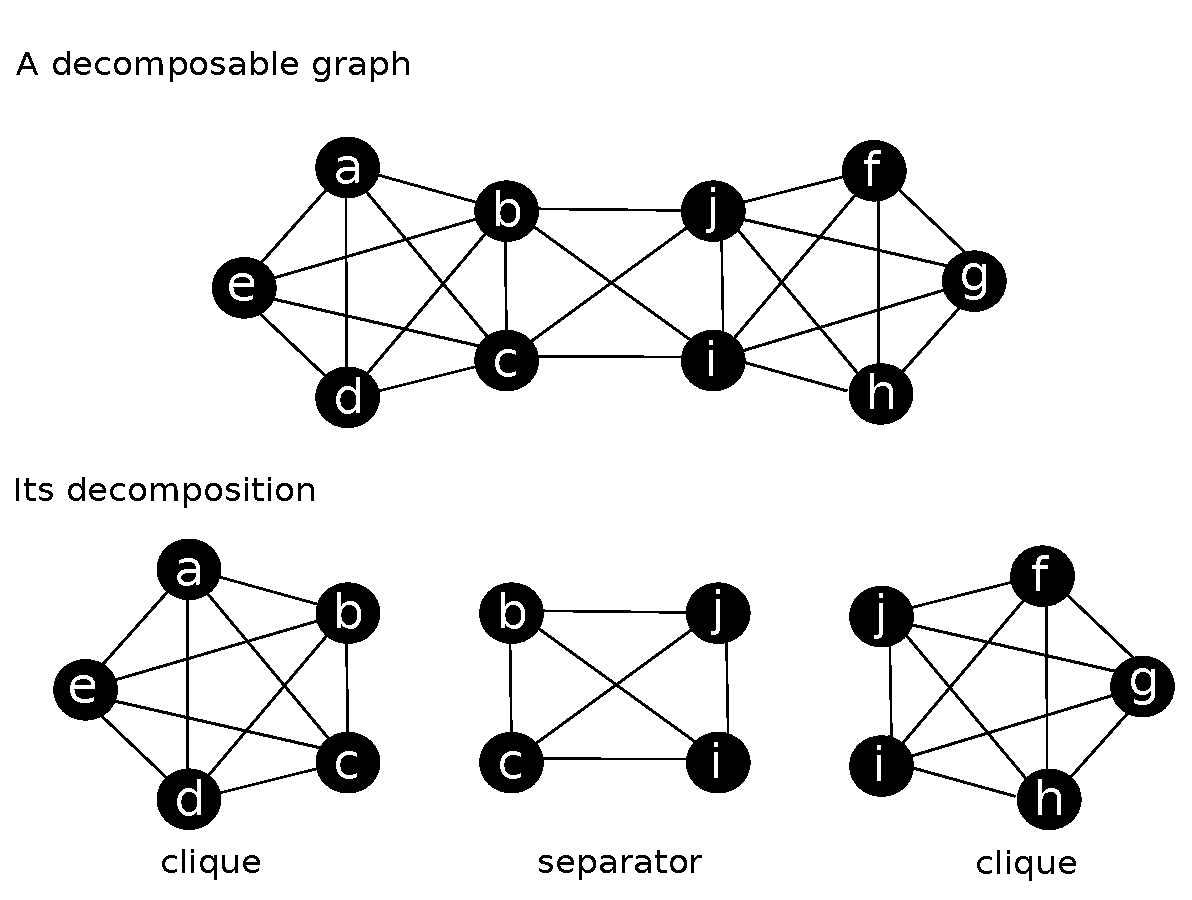
\includegraphics[angle=0, scale=0.45]{DecomposableGraph.eps}
\end{center}
\caption{The top row shows a decomposable graph. The bottom row displays its decomposition in terms of the two cliques, comprising vertices $\{a, b, c, d, e\}$ and $\{f, g, h, i, j\}$ and the edges connecting them, and a separator with vertices $\{b, c, i, j\}$ and the edges connecting them.
\label{fig.decomposableGraphIllustration}}
\end{figure}

\begin{figure}[h!]
\centering
\begin{tabular}{ll}
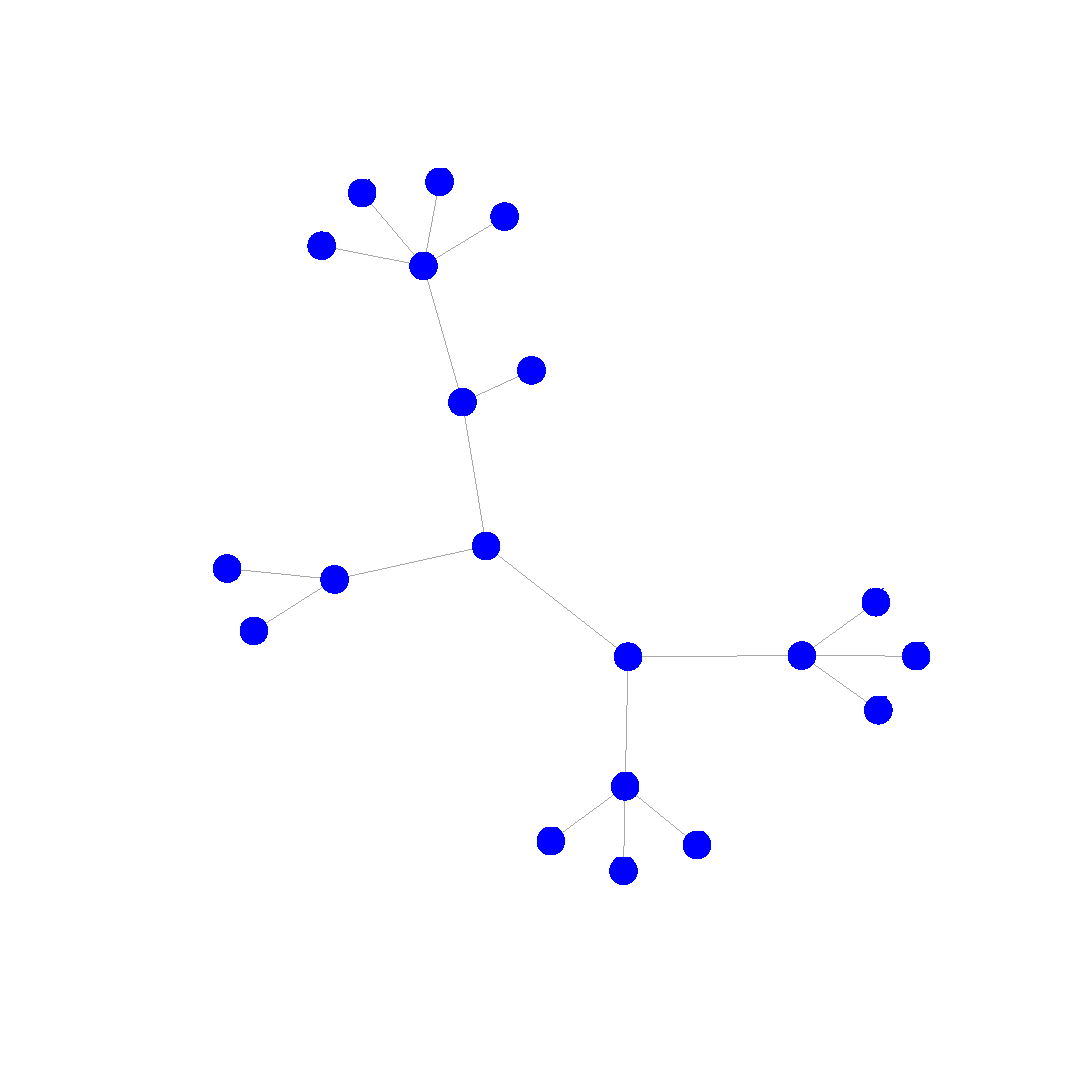
\includegraphics[angle=0, scale=0.4]{chordalGraph_tree_graph.eps} &
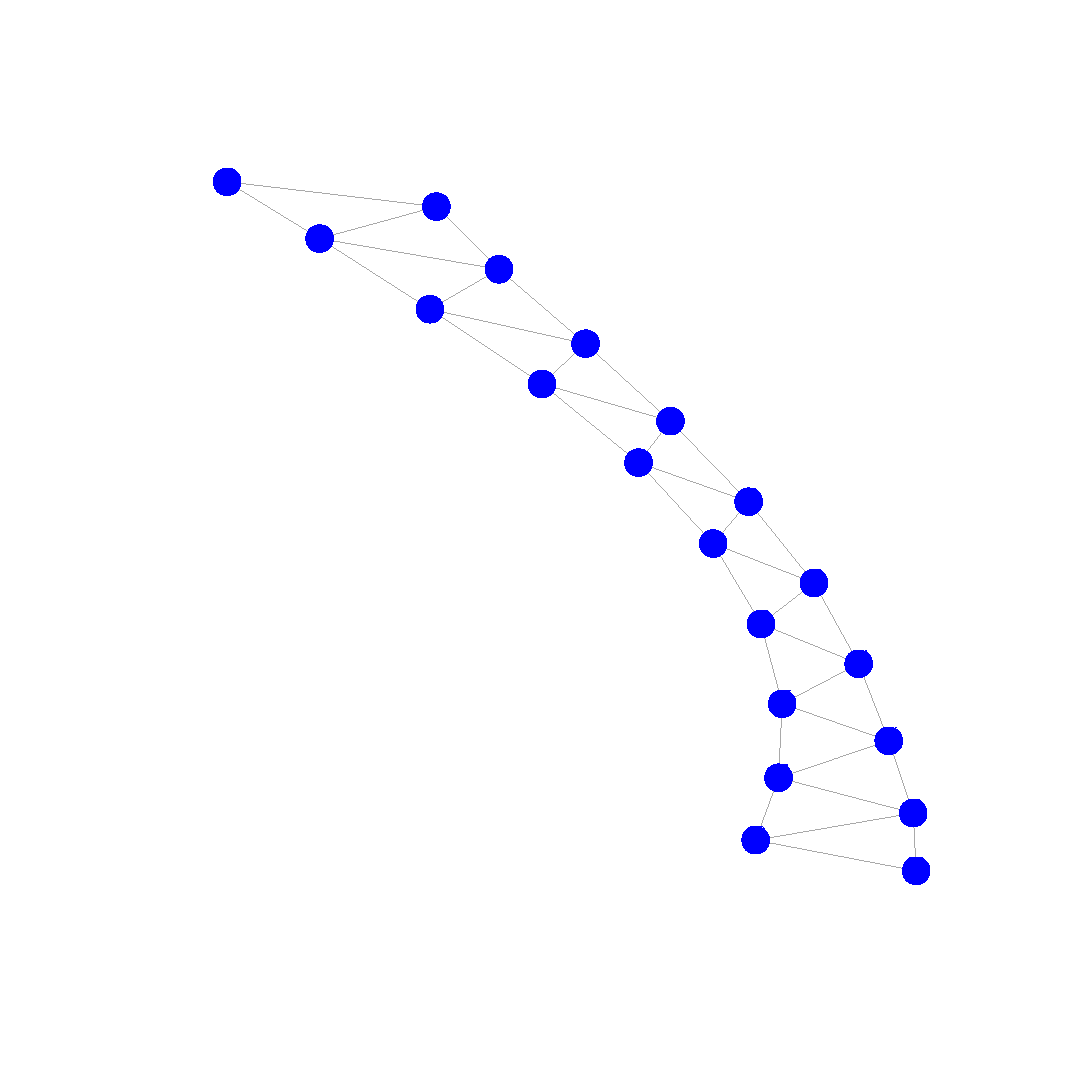
\includegraphics[angle=0, scale=0.4]{chordalGraph_chain_graph.eps}
\end{tabular}
\caption{Two examples of decomposable graphs: the tree and a chain graph. }
\label{figSM:examplesOfChordalGraph}
\end{figure}



\newpage
\section*{SM IV: initial estimate of $\mathbf{\Omega}$ with chordal support}
Under the assumption of a decomposable conditional independence graph $\mathcal{G}$, the ridge ML estimator of $\mathbf{\Omega}_{\varepsilon}$ can be expressed in limiting cases ($\lambda_{\omega}=0$, $\lambda_{\omega}=\infty$ and $\mathcal{S} = \emptyset$) as a combination of the ridge ML estimators of the cliques and separators that decompose $\mathcal{G}$. Fully analogous to unpenalized case specified by Proposition 5.9 of \cite{Laur1996} but with the unpenalized marginal ML covariance estimates of cliques and separators replaced by their penalized counterparts.

To derive the ridge ML estimator for the aforementioned limiting cases, note by direct observation that the decomposability of the support of $\mathbf{\Omega}_{\varepsilon}$ implies:
\begin{eqnarray}
\nonumber
\mbox{tr}  [ (\mathbf{\Omega}_{\varepsilon} - \mathbf{\Omega}_0)^\top (\mathbf{\Omega}_{\varepsilon} - \mathbf{\Omega}_0)]
& = & \sum_{\mathsfit{C} \in \mathcal{C}} \mbox{tr} \{ [ (\mathbf{\Omega}_{\varepsilon})_{\mathsfit{C},\mathsfit{C}} - (\mathbf{\Omega}_0)_{\mathsfit{C}, \mathsfit{C}} ]^{\top} [(\mathbf{\Omega}_{\varepsilon})_{\mathsfit{C},\mathsfit{C}} - (\mathbf{\Omega}_0)_{\mathsfit{C}, \mathsfit{C}}] \}
\\
\label{form.reformulatedRidgePanelty}
& &  \, - \, \sum_{\mathsfit{S} \in \mathcal{S}} \mbox{tr} \{ [ (\mathbf{\Omega}_{\varepsilon})_{\mathsfit{S},\mathsfit{S}} - (\mathbf{\Omega}_0)_{\mathsfit{S}, \mathsfit{S}} ]^{\top} [(\mathbf{\Omega}_{\varepsilon})_{\mathsfit{S}, \mathsfit{S}} - (\mathbf{\Omega}_0)_{\mathsfit{S}, \mathsfit{S}}] \},
\end{eqnarray}
in which $\mathbf{\Omega}_0$ is assumed to share its support with $\mathbf{\Omega}_{\varepsilon}$. For square, symmetric $\mathbf{S}_{\varepsilon} \succeq$, $\mathbf{\Omega}_{\varepsilon} \succ 0$, and $\mathbf{\Omega}_0 \succ 0$ of arbitrary but equal dimensions define
\begin{eqnarray*}
\mathcal{L}_{\omega}^{\mbox{{\tiny pen}}}(\mathbf{S}_{\varepsilon}, \mathbf{\Omega}_{\varepsilon}, \mathbf{\Omega}_0, \lambda_{\omega}) & = & \frac{1}{2} n (\mathcal{T} - 1) \big\{ \log| \mathbf{\Omega}_{\varepsilon} |   - \mbox{tr}  ( \mathbf{S}  \mathbf{\Omega}_{\varepsilon} ) - \lambda_{\omega} \mbox{tr}  [ (\mathbf{\Omega}_{\varepsilon} -\mathbf{\Omega}_0)^{\top} (\mathbf{\Omega}_{\varepsilon} - \mathbf{\Omega}_0) ] \big\}.
\end{eqnarray*}
Using the reformulated ridge penalty (\ref{form.reformulatedRidgePanelty}) together with iterative application of Lemma 5.5. of \cite{Laur1996}, which decomposes the unpenalized log-likelihood in a linear combination of those of the cliques and separators, the loss function for $\mathbf{\Omega}_{\varepsilon}$ can then be rewritten to:
\begin{eqnarray} \label{form.decomposedPenLoglik}
\sum_{\mathsfit{C} \in \mathcal{C}} \mathcal{L}^{\mbox{{\tiny pen}}}_{\omega}[(\mathbf{S}_{\varepsilon})_{\mathsfit{C},\mathsfit{C}}, (\mathbf{\Omega}_{\varepsilon})_{\mathsfit{C},\mathsfit{C}}, (\mathbf{\Omega}_{0})_{\mathsfit{C},\mathsfit{C}}, \lambda_{\omega}] - \sum_{\mathsfit{S} \in \mathcal{S}} \nu(\mathsfit{S}) \mathcal{L}^{\mbox{{\tiny pen}}}_{\omega} [(\mathbf{S}_{\varepsilon})_{\mathsfit{S},\mathsfit{S}}, (\mathbf{\Omega}_{\varepsilon})_{\mathsfit{S},\mathsfit{S}},
(\mathbf{\Omega}_{0})_{\mathsfit{S},\mathsfit{S}}, \lambda_{\omega}],
\end{eqnarray}
where $\nu(\mathsfit{S})$ is the number of times separator $\mathsfit{S}$ forms the intersection of two neighboring cliques.

Recall from the main text that, when $\mathcal{G}$ decomposes into cliques $\mathsfit{C}_1$, $\mathsfit{C}_2$ and $\mathsfit{S}$, the proposed ridge ML estimator is:
\begin{eqnarray*}
\widehat{\mathbf{\Omega}}_{\varepsilon}(\lambda_{\omega}) & = &
\left(
\begin{array}{lll}
\, [\widehat{\mathbf{\Omega}}_{\varepsilon}^{({\mathsfit{C}_1})}(\lambda_{\omega})]_{\mathsfit{C}_1 \setminus \mathsfit{S}, \mathsfit{C}_1 \setminus \mathsfit{S}} & [\widehat{\mathbf{\Omega}}_{\varepsilon}^{({\mathsfit{C}_1})}(\lambda_{\omega})]_{\mathsfit{C}_1 \setminus \mathsfit{S}, \mathsfit{S}} & \mathbf{0}_{|\mathsfit{C}_1 \setminus \mathsfit{S}| \times |\mathsfit{C}_2 \setminus \mathsfit{S}|}
\\
\, [\widehat{\mathbf{\Omega}}_{\varepsilon}^{(\mathsfit{C}_1)}(\lambda_{\omega})]_{\mathsfit{S}, \mathsfit{C}_1 \setminus \mathsfit{S}} & [\widehat{\mathbf{\Omega}}_{\varepsilon}^{({\mathsfit{C}_1})}(\lambda_{\omega})]_{\mathsfit{S}, \mathsfit{S}} + [\widehat{\mathbf{\Omega}}_{\varepsilon}^{({\mathsfit{C}_2})}(\lambda_{\omega})]_{\mathsfit{S}, \mathsfit{S}} - \widehat{\mathbf{\Omega}}_{\varepsilon}^{(\mathsfit{S})}(\lambda_{\omega}) & [\widehat{\mathbf{\Omega}}_{\varepsilon}^{({\mathsfit{C}_2})}(\lambda_{\omega})]_{\mathsfit{S}, \mathsfit{C}_2 \setminus \mathsfit{S}}
\\
\, \mathbf{0}_{|\mathsfit{C}_2 \setminus \mathsfit{S}| \times |\mathsfit{C}_1 \setminus \mathsfit{S}|} & [\widehat{\mathbf{\Omega}}_{\varepsilon}^{({\mathsfit{C}_2})}(\lambda_{\omega})]_{\mathsfit{C}_2 \setminus \mathsfit{S}, \mathsfit{S}} & [\widehat{\mathbf{\Omega}}_{\varepsilon}^{({\mathsfit{C}_2})}(\lambda_{\omega})]_{\mathsfit{C}_2 \setminus \mathsfit{S}, \mathsfit{C}_2 \setminus \mathsfit{S}}
\end{array}
\right),
\end{eqnarray*}
where $\widehat{\mathbf{\Omega}}_{\varepsilon}^{({\mathsfit{C}_1})}(\lambda_{\omega})$, $\widehat{\mathbf{\Omega}}_{\varepsilon}^{({\mathsfit{C}_1})}(\lambda_{\omega})$ and $\widehat{\mathbf{\Omega}}_{\varepsilon}^{({\mathsfit{S}})}(\lambda_{\omega})$ are the marginal ridge ML covariance estimators for cliques $\mathsfit{C}_1$, $\mathsfit{C}_2$ and separator $\mathsfit{S}$. Note that each of these marginal estimator satisfy the marginal estimating equation, e.g.:
\begin{eqnarray*}
[\widehat{\mathbf{\Omega}}_{\varepsilon}^{({\mathsfit{C}_1})}(\lambda_{\omega})]^{-1} - \lambda_{\omega} \widehat{\mathbf{\Omega}}_{\varepsilon}^{({\mathsfit{C}_1})}(\lambda_{\omega}) & = & (\mathbf{S}_{\varepsilon})_{\mathsfit{C}_1, \mathsfit{C}_1} - \lambda_{\omega} (\mathbf{\Omega}_{0})_{\mathsfit{C}_1, \mathsfit{C}_1},
\end{eqnarray*}
confer \cite{VWie2014b} for details.


To show that this estimator maximizes (in the three limiting cases) the ridge penalized log-likelihood under the assumption of a decomposable conditional independence graph, we study this penalized log-likelihood in the vicinity of the proposed estimator. Let a $\mathbf{\Delta}$ be a $p \times p$ dimensional matrix and $\gamma$ a constant close to but unequal to zero. Consider a single summand of the penalized log-likelihood (\ref{form.decomposedPenLoglik}), say, that of the first clique. It may then, after noting that $\log(\mathbf{A} + \varepsilon \mathbf{B}) = \log( \mathbf{A}) + \varepsilon \mathbf{A}^{-1} \mathbf{B} + \mathcal{O}(\varepsilon^2)$ and $\log( | \mathbf{A} |)  = \mbox{tr} [ \log(\mathbf{A})]$, be approximated by:
\begin{eqnarray*}
& & \hspace{-1cm} \mathcal{L}^{\mbox{{\tiny pen}}}_{\omega} \big\{ (\mathbf{S}_{\varepsilon})_{\mathsfit{C}_1,\mathsfit{C}_1}, [\widehat{\mathbf{\Omega}}_{\varepsilon}(\lambda_{\omega}) ]_{\mathsfit{C}_1,\mathsfit{C}_1} + \gamma \, (\mathbf{\Delta})_{\mathsfit{C}_1,\mathsfit{C}_1}, (\mathbf{\Omega}_{0})_{\mathsfit{C}_1,\mathsfit{C}_1}, \lambda_{\omega} \big\}
\\
& \approx & \log \big\{ | [\widehat{\mathbf{\Omega}}_{\varepsilon}(\lambda_{\omega}) ]_{\mathsfit{C}_1,\mathsfit{C}_1} | \big\}
 - \, \mbox{tr}  \big\{ (\mathbf{S}_{\varepsilon})_{\mathsfit{C}_1,\mathsfit{C}_1}  [\widehat{\mathbf{\Omega}}_{\varepsilon}(\lambda_{\omega})]_{\mathsfit{C}_1,\mathsfit{C}_1} \big\}
\\
& &
- \frac{1}{2} \lambda_{\omega} \mbox{tr}  \Big(  \big\{ [\widehat{\mathbf{\Omega}}_{\varepsilon}(\lambda_{\omega})]_{\mathsfit{C}_1,\mathsfit{C}_1} - (\mathbf{\Omega}_{0})_{\mathsfit{C}_1,\mathsfit{C}_1} \big\}^{\top} \big\{ [\widehat{\mathbf{\Omega}}_{\varepsilon}(\lambda_{\omega})]_{\mathsfit{C}_1,\mathsfit{C}_1} - (\mathbf{\Omega}_{0})_{\mathsfit{C}_1,\mathsfit{C}_1} \big\} \Big)
\\
& & + \, \gamma \, \mbox{tr} \Big[ \Big(
\big\{ [\widehat{\mathbf{\Omega}}_{\varepsilon}(\lambda_{\omega})]_{\mathsfit{C}_1,\mathsfit{C}_1} \big\}^{-1} -
\big\{ [\widehat{\mathbf{\Omega}}_{\varepsilon}(\lambda_{\omega})]^{-1} \big\}_{\mathsfit{C}_1,\mathsfit{C}_1}
\Big) ( \mathbf{\Delta})_{\mathsfit{C}_1,\mathsfit{C}_1} \Big) \Big]
\\
& & - \frac{1}{2} \gamma^2 \lambda_{\omega} \mbox{tr}  \big\{  [  (\mathbf{\Delta})_{\mathsfit{C}_1,\mathsfit{C}_1} ]^{\top}  ( \mathbf{\Delta})_{\mathsfit{C}_1,\mathsfit{C}_1}  \big\},
\end{eqnarray*}
in which we also used the estimating equation.

Only the latter two summands of this approximation of the penalized log-likelihood of the clique involve $\gamma$. Now consider the three boundary cases separately:
\begin{compactitem}
\item When $\lambda_{\omega} = 0$ the summands in the approximation stemming from the penalty vanish and the claim is warranted by Lemma 5.5 of \cite{Laur1996}.

\item When $\mathcal{S} = \emptyset$, the precision matrix is block diagonal and the blocks can be estimated marginally. This implies $[(\widehat{\mathbf{\Omega}}_{\varepsilon})_{\mathsfit{C}_1,\mathsfit{C}_1} ]^{-1} =
[(\widehat{\mathbf{\Omega}}_{\varepsilon})^{-1}]_{\mathsfit{C}_1,\mathsfit{C}_1}$ and ensures that the first summand involving $\gamma$ vanishes. As the second summand can only contribute negatively to the log-likelihood for any $\gamma \not= 0$, the proposed estimator maximizes the log-likelihood.

\item When $\lambda_{\omega}$ tends to infinity, the second summand involving $\gamma$ dominates the other. For these dominant summands:
\begin{eqnarray*}
\mbox{tr}  ( \mathbf{\Delta}^\top \mathbf{\Delta})
& = & \sum_{\mathsfit{C} \in \mathcal{C}} \mbox{tr} \{ [ (\mathbf{\Delta})_{\mathsfit{C},\mathsfit{C}}]^{\top} (\mathbf{\Delta})_{\mathsfit{C},\mathsfit{C}} \}
\, - \, \sum_{\mathsfit{S} \in \mathcal{S}} \mbox{tr} \{ [ (\mathbf{\Delta})_{\mathsfit{S},\mathsfit{S}}]^{\top} (\mathbf{\Delta})_{\mathsfit{S}, \mathsfit{S}} \}.
\end{eqnarray*}
The total contribution of these terms to the log-likelihood is thus negative for any choice of $\gamma$ other than zero.

\end{compactitem}
Hence, the proposed estimator indeed maximizes the penalized log-likelihood in the three limiting cases.

\newpage
\section*{SM V: Path analysis illustration}
The path analysis of autocovariance is illustrated by means of a toy example. Consider a VAR(1) model parametrized by:
\begin{eqnarray*}
\mathbf{\nu} \, \, \, = \, \, \,
\left(
\begin{array}{rrr}
0
\\
0
\\
0
\end{array}
\right),
\quad \mathbf{A} \, \, \, = \, \, \,
\left(
\begin{array}{rrr}
\rfrac{1}{2} & \rfrac{1}{2} & \rfrac{1}{2}
\\
0 & 0 & 0
\\
0 & 0 & 0
\end{array}
\right)
\quad \mbox{ and } \quad
\mathbf{\Sigma}_{\varepsilon} & = &
\left(
\begin{array}{rrr}
1 & \rfrac{1}{5} & \rfrac{1}{5}
\\
\rfrac{1}{5} & 1 & 0
\\
\rfrac{1}{5} & 0 & 1
\end{array}
\right)^{-1}.
\end{eqnarray*}
The top row of Figure \ref{fig.TSCGpathAnalysis} displays the corresponding time series chain graph.

The autocovariance between $Y_{1,t}$ and $Y_{1,t+1}$ (dropping the sample index for notational clarity) is: $\mbox{Cov}(Y_{1,t}, Y_{1,t+1}) = (\mathbf{\Sigma}_{\varepsilon} \mathbf{A}^{\top})_{1,1} = 0.326087$. From the time series chain graph it is immediate that $Y_{1,t}$ and $Y_{1,t+1}$  are connected by three paths (visualized by the bottom row of Figure \ref{fig.TSCGpathAnalysis}): \textit{i)} $Y_{1,t} \rightarrow Y_{1,t+1}$, \textit{ii)} $Y_{1,t} \rightarrow Y_{2,t} \rightarrow Y_{1,t+1}$, and \textit{iii)} $Y_{1,t} \rightarrow Y_{3,t} \rightarrow Y_{1,t+1}$. The	 covariance between $Y_{1,t}$ and $Y_{1,t+1}$ can now be decomposed into the contributions of each of these paths. Using the decomposition of the autocovariance in terms of the paths' contributions from the main text one obtains: $0.5434783$ (for $Y_{1,t} \rightarrow Y_{1,t+1}$), $-0.1086957$ (for $Y_{1,t} \rightarrow Y_{2,t} \rightarrow Y_{1,t+1}$) and $-0.1086957$ (for $Y_{1,t} \rightarrow Y_{3,t} \rightarrow Y_{1,t+1}$). These contributions indeed sum to $0.326087$, which equals $\mbox{Cov}(Y_{1,t}, Y_{1,t+1})$.

\begin{figure}[b!]
\begin{center}
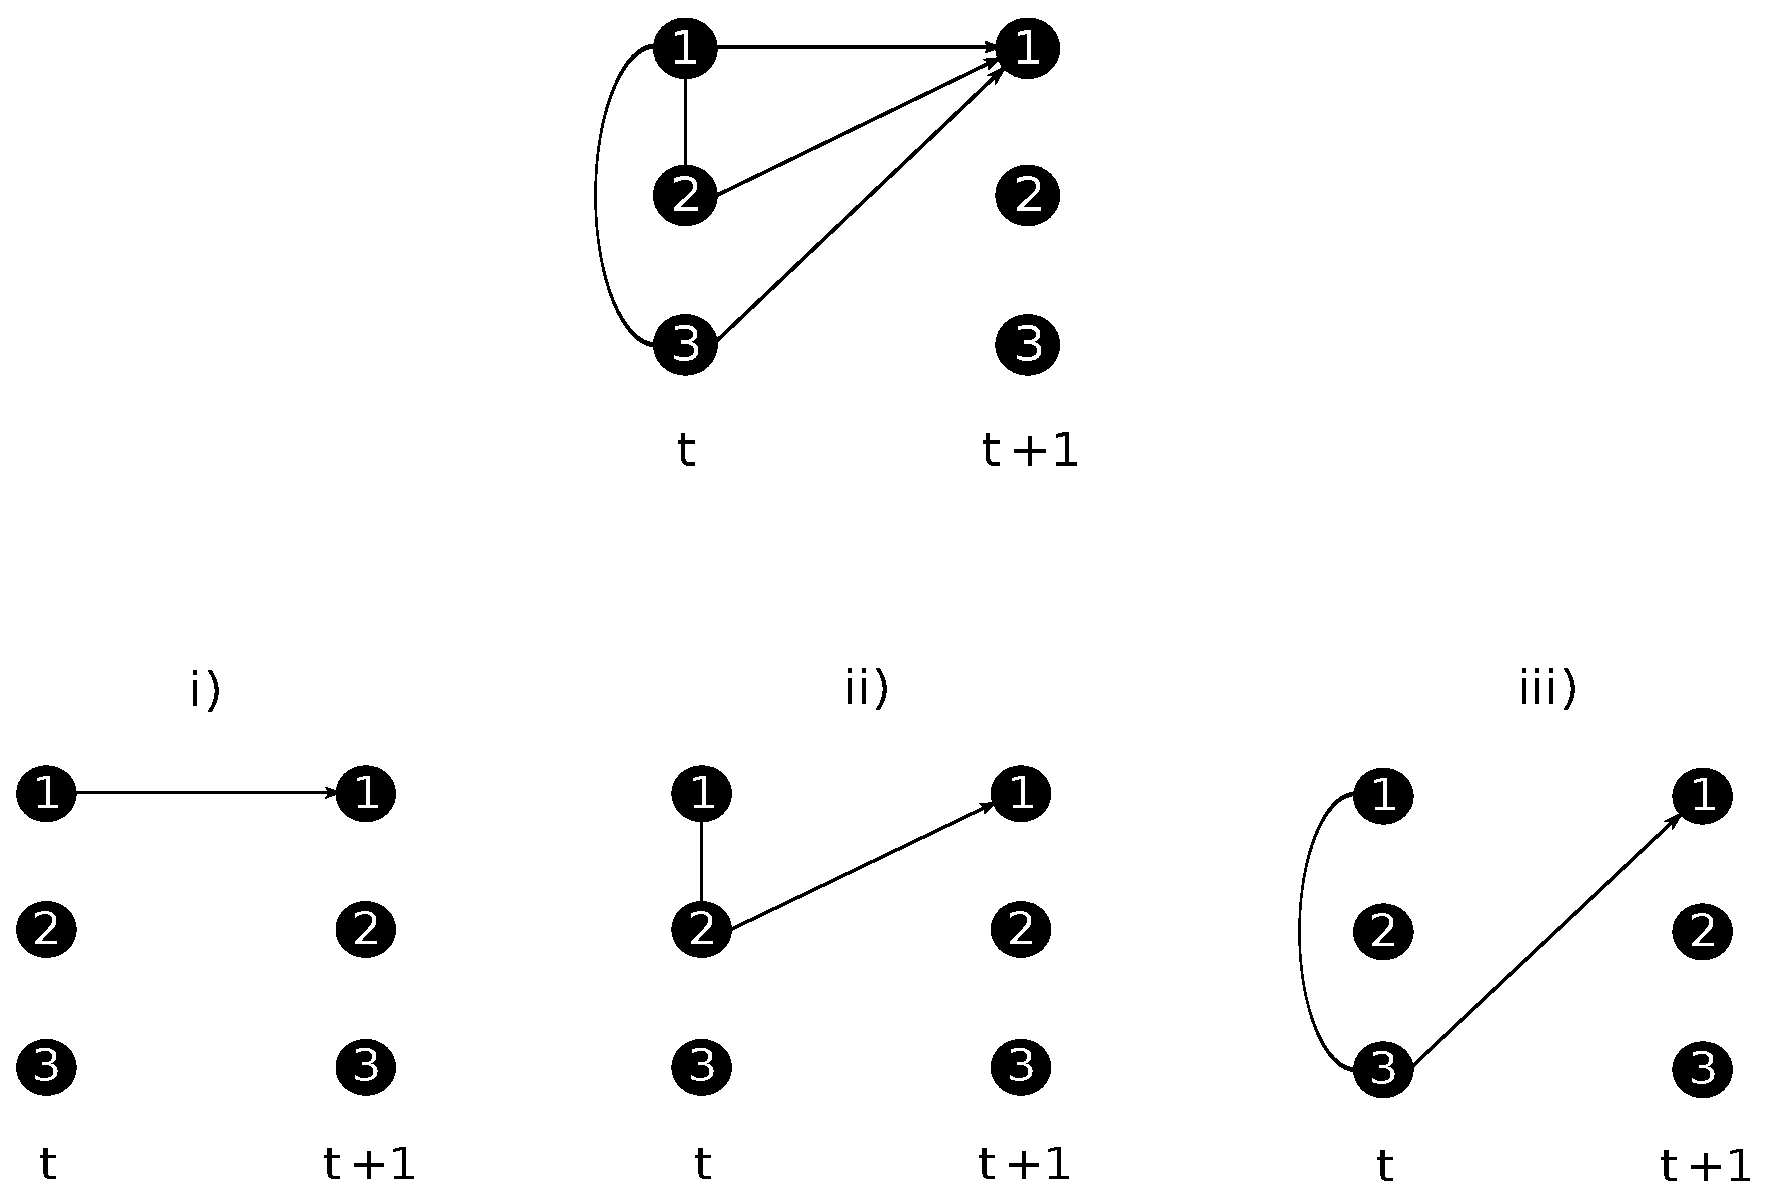
\includegraphics[angle=0, scale=0.5]{TSCG_pathExample2.eps}
\end{center}
\caption{The top row shows the time series chain graph of the toy model. The bottom row displays the three paths in the time series chain graph connecting the first variate between to consecutive time points.
\label{fig.TSCGpathAnalysis}}
\end{figure}



\newpage
\section*{SM VI: Design of time-course studies in GEO}
\cite{Ernst2005} observed that more than $80\%$ of time-course gene expression microarray data sets have 8 or fewer number of time points. This reference being somewhat out of date, we conducted our own survey using the GEO data base \cite{Edga2002}. Using the search terms ``time course'', ``cancer'', ``human'',  ``cell line'', ``gene expression'', ``microarray'', 85 studies where selected (at June 23, 2015). From the resulting list we excluded studies involving hematological tumors and data set GSE762 with a rather intricate experimental design (among other a time component). Finally, 63 studies satisfy these criteria, involving cell lines of various cancer types (breast, colon, prostate, ovarian, kidney and lung) and were mainly conducted using Affymetrix gene expression arrays (confer Table \ref{tableSM:GEOdatasets}). Figure \ref{figSM:GEOhist} shows histograms of the number of time-points $\mathcal{T}$ and individuals $n$ (left panels) and the scatterplot of these study characteristics. From the provided table and histograms we conclude that a reasonable optimistic and simultaneously empirically maximum number of time-points and individuals are 10 and 5, respectively.
\\
\mbox{ }
\\
\mbox{ }
\\
\mbox{ }

\begin{figure}[h!]
\centering
\begin{tabular}{ccc}
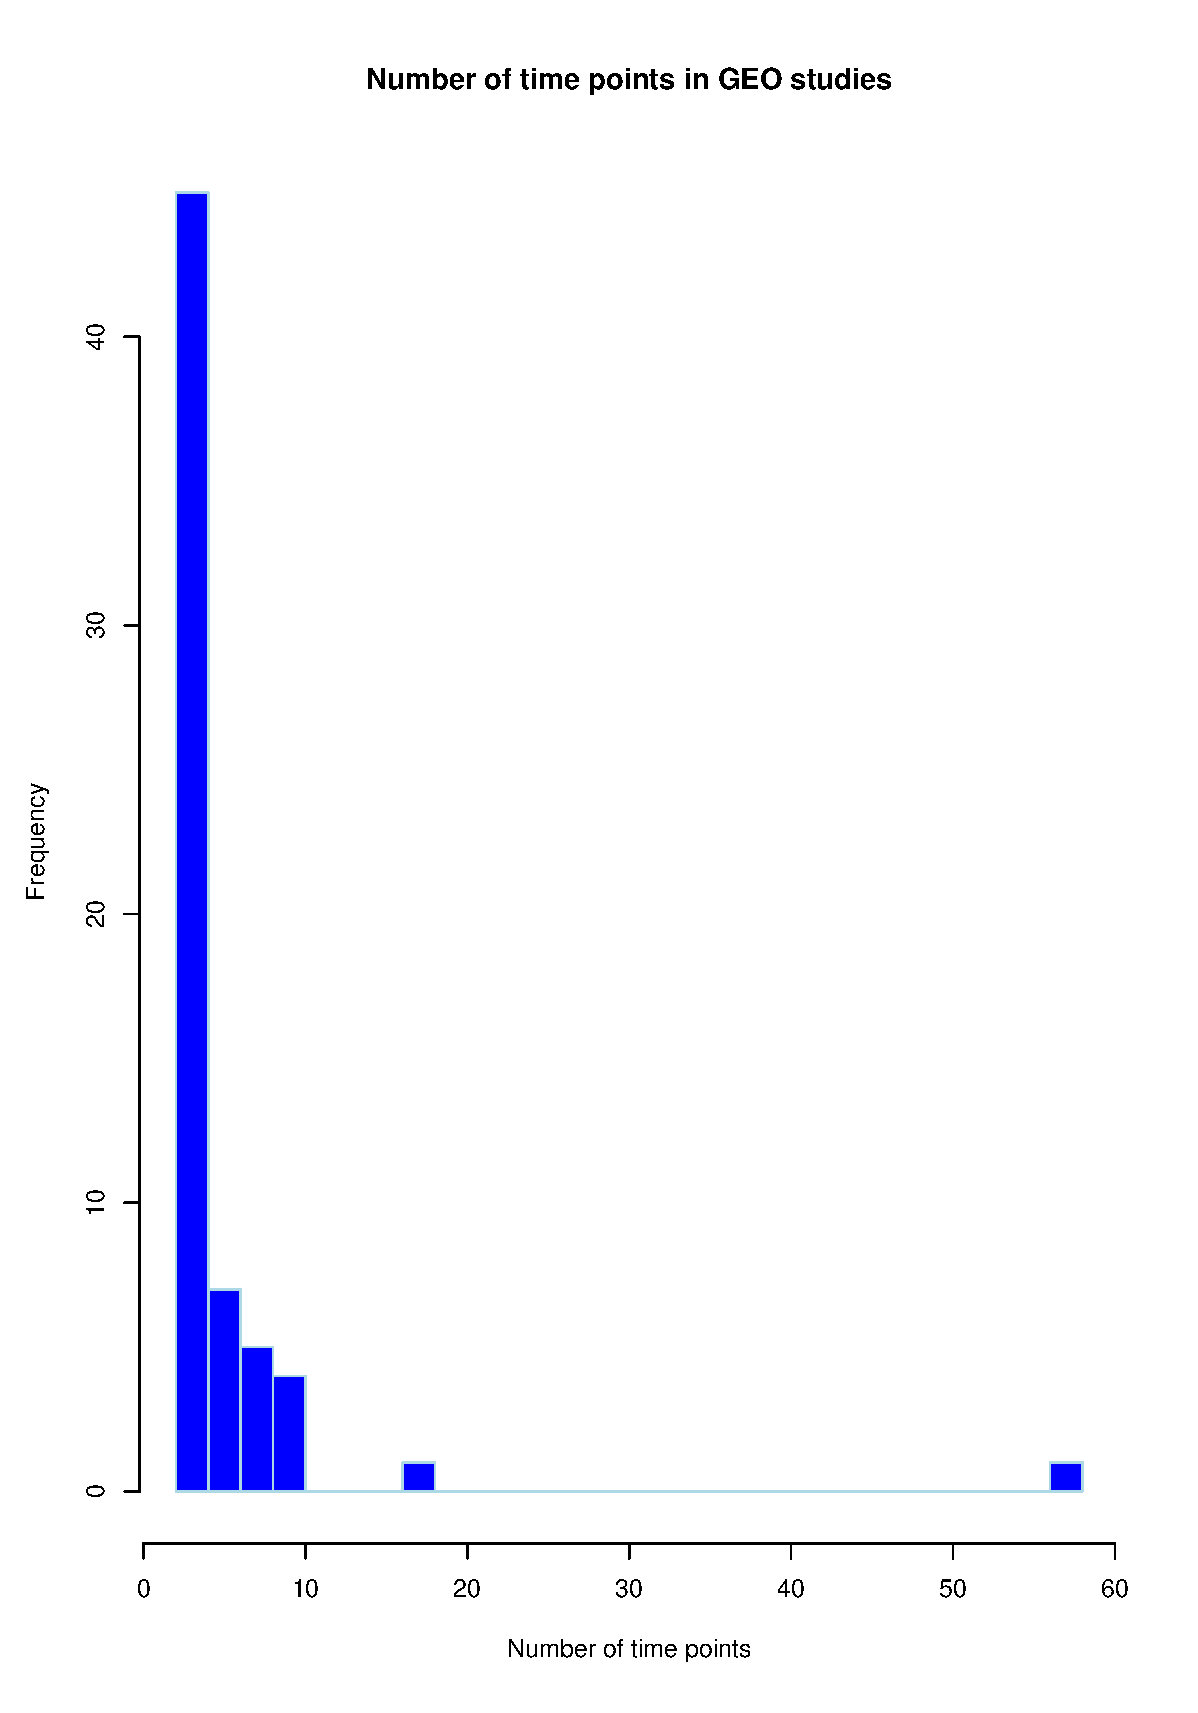
\includegraphics[scale=0.24]{GEOtime.eps} &
\includegraphics[scale=0.24]{GEOind.eps} &
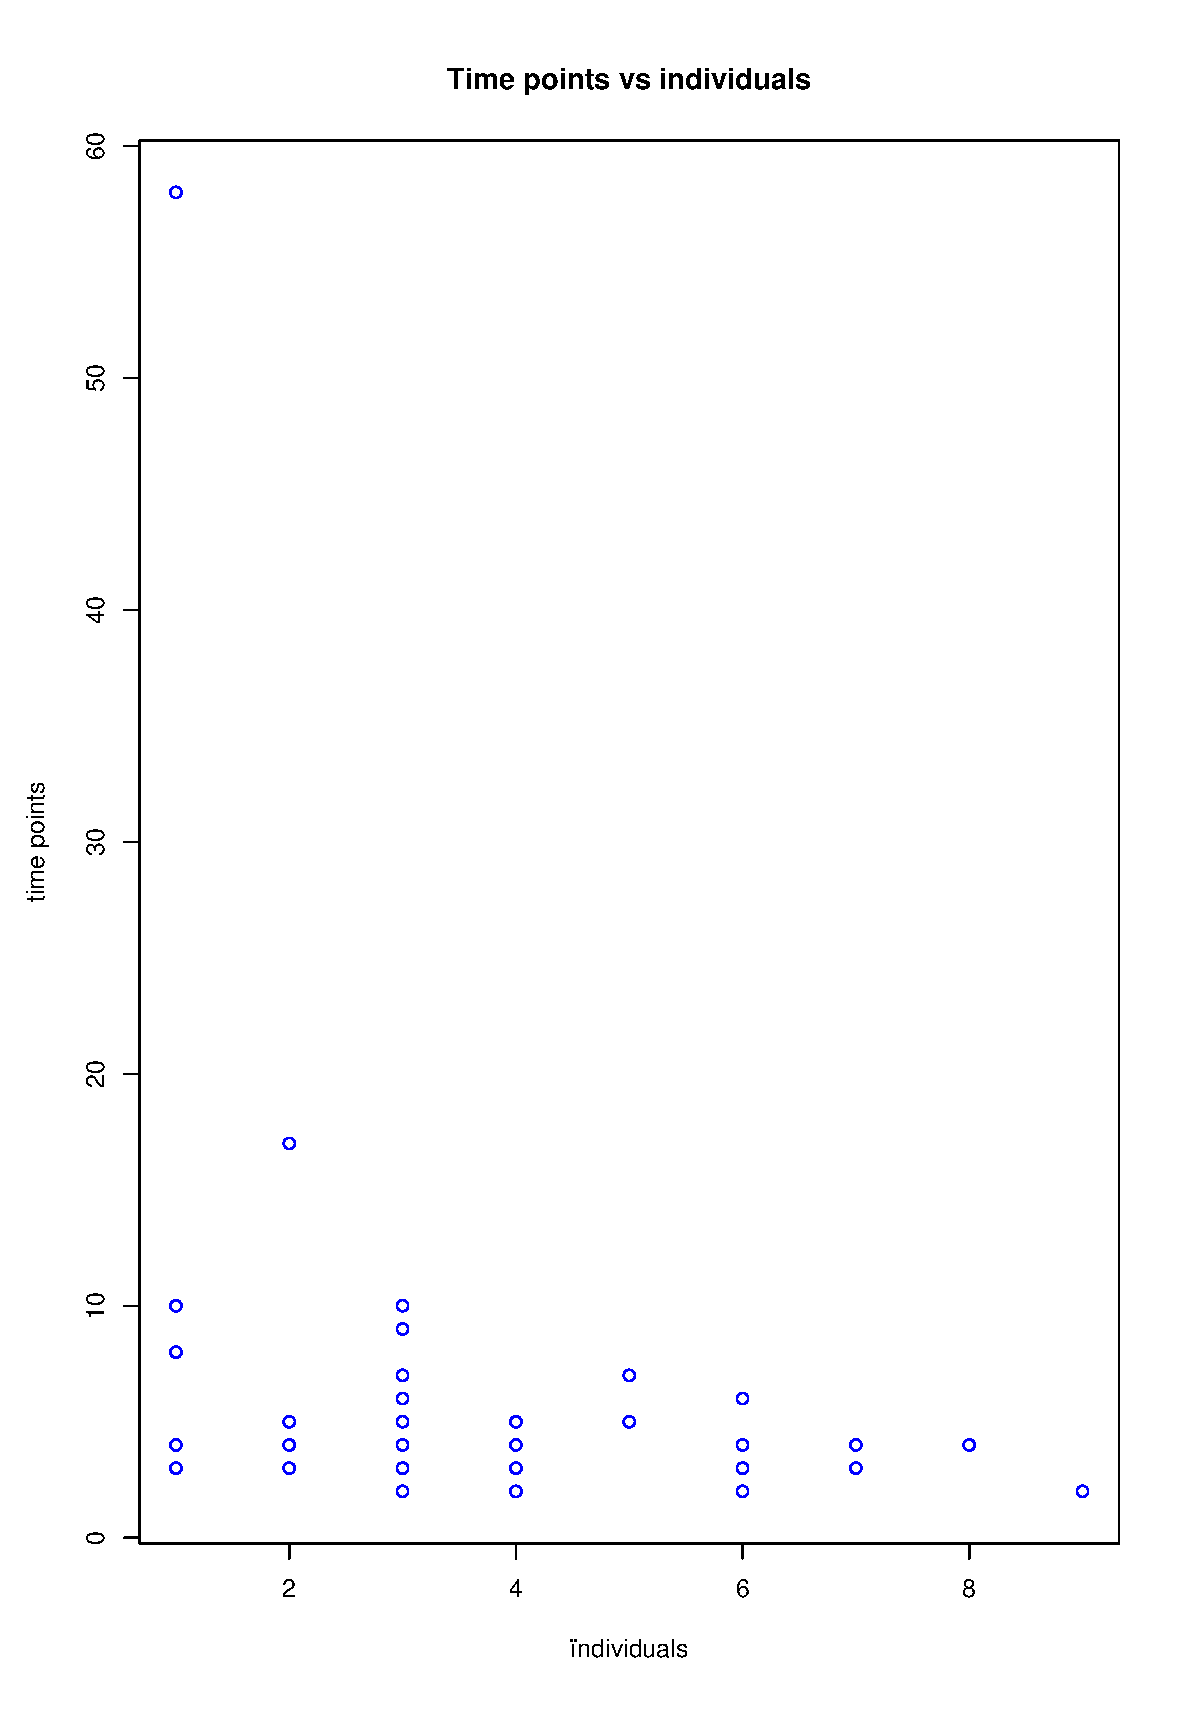
\includegraphics[scale=0.24]{GEOscat.eps}\\
\end{tabular}
\caption{Number of time-points and observations in microarray time-course gene expression studies from GEO database. Left panel presents the histogram of number of time-points, while the middle panel shows the histogram of the number of observations (cell lines) in GEO studies. The right panel plots the number of time points against the number of individuals.}
\label{figSM:GEOhist}
\end{figure}



% Histograms of the number of time-points (left panel) and observations (right panel) of GEO  gene expression microarray studies with a time-course set-up.




\begin{table}
{\scriptsize
\begin{tabular}{lrrrlll}
\hline
& & & & & & \\
\textbf{data}	&	\textbf{\# time}	&	\textbf{\# individuals}	&	\textbf{\# treatments}	&	\textbf{cancer}	&	\textbf{organism}	&	\textbf{platform}	\\
\textbf{set ID}	&	\textbf{points}	&		&	&	\textbf{type}	&		& \\
& & & & & &
\\
\hline
& & & & & &
\\
GSE7868	&	3	&	3	&	1	&	prostate	&	human	&	Affymetrix	\\
GDS2626	&	4	&	7	&	2	&	breast	&	human	&	Affymetrix	\\
GSE29917	&	7	&	5	&	3	&	breast	&	human	&	Agilent	\\
GSE13009	&	17	&	2	&	2	&	breast	&	human	&	Affymetrix	\\
GDS4367	&	5	&	3	&	1	&	colon	&	mouse	&	Affymetrix	\\
GDS4121	&	3	&	1	&	1	&	prostate	&	human 	&	Affymetrix	\\
GDS4110	&	9	&	3	&	1	&	prostate	&	human	&	Affymetrix	\\
GDS4063	&	2	&	9	&	3	&	breast	&	human	&	Affymetrix	\\
GDS4052	&	2	&	6	&	3	&	breast	&	human	&	Affymetrix	\\
GDS3910	&	3	&	2	&	3	&	breast	&	human	&	Affymetrix	\\
GDS3887	&	4	&	4	&	2	&	bladder	&	mouse	&	Affymetrix	\\
GDS3872	&	3	&	3	&	2	&	ovarian	&	human	&	Affymetrix	\\
GDS3761	&	3	&	4	&	2	&	prostate	&	human	&	Affymetrix	\\
GDS3710	&	9	&	3	&	1	&	epithelial	&	human	&	Affymetrix	\\
GDS3517	&	4	&	3	&	4	&	melanoma	&	human	&	Affymetrix	\\
GDS3484	&	2	&	3	&	2	&	breast	&	human	&	Affymetrix	\\
GDS3792	&	3	&	2	&	2	&	ovarian	&	human	&	Affymetrix	\\
GDS3358	&	5	&	2	&	2	&	prostate	&	human	&	Affymetrix	\\
GDS3319	&	3	&	1	&	3	&	thyroid	&	human	&	Affymetrix	\\
GDS3285	&	4	&	3	&	1	&	breast	&	human 	&	Affymetrix	\\
GDS3283	&	2	&	6	&	2	&	breast	&	human	&	Affymetrix	\\
GDS3116	&	58	&	1	&	2	&	breast	&	human	&	Affymetrix	\\
GDS3111	&	3	&	3	&	2	&	prostate	&	human	&	Affymetrix	\\
GDS2975	&	4	&	2	&	1	&	ovarian	&	human	&	Affymetrix	\\
GDS2810	&	3	&	2	&	2	&	breast	&	human	&	Affymetrix	\\
GDS2604	&	6	&	6	&		&	lung	&	human 	&	Affymetrix	\\
GDS2323	&	3	&	3	&	1	&	breast	&	human 	&	Affymetrix	\\
GDS2097	&	4	&	1	&	2	&	breast	&	human 	&	Affymetrix	\\
GDS2096	&	4	&	1	&	2	&	breast	&	human 	&	Affymetrix	\\
GDS1942	&	8	&	1	&	2	&	colon	&	human	&	Affymetrix	\\
GDS1736	&	2	&	4	&	2	&	prostate	&	human	&	Affymetrix	\\
GDS1627	&	3	&	2	&		&	breast	&	human	&	oligo	\\
GDS848	&	3	&	7	&	3	&	breast	&	human	&	oligo	\\
GDS725	&	10	&	1	&	1	&	prostate	&	human	&	Affymetrix	\\
GDS719	&	4	&	2	&	3	&	prostate	&	human	&	Affymetrix	\\
GDS528	&	3	&	3	&	1	&	colon	&	human	&	Affymetrix	\\
GSE41828	&	5	&	5	&	2	&	prostate	&	human	&	Affymetrix	\\
GSE41680	&	4	&	1	&	2	&	melanoma	&	human	&	Affymetrix	\\
GSE31128	&	4	&	3	&	4	&	breast	&	human 	&	Illumina	\\
GSE28305	&	4	&	2	&	1	&	breast	&	human	&	Affymetrix	\\
GDS4853	&	4	&	3	&	2	&	stomach	&	human	&	Affymetrix	\\
GSE26834	&	2	&	3	&	6	&	breast	&	human	&	Affymetrix	\\
GSE23616	&	3	&	3	&	2	&	ovarian	&	human	&	Affymetrix	\\
GSE20361	&	8	&	1	&	1	&	breast	&	human	&	Affymetrix	\\
GSE23845	&	4	&	4	&	1	&	bladder	&	human	&	Affymetrix	\\
GSE15947	&	3	&	4	&	3	&	prostate	&	human	&	Affymetrix	\\
GSE18494	&	4	&	3	&	3	&	breast	&	human	&	Affymetrix	\\
GSE17708	&	10	&	3	&	2	&	lung	&	human	&	Affymetrix	\\
GSE11428	&	3	&	3	&	6	&	prostate	&	human	&	Affymetrix	\\
GSE16424	&	4	&	6	&	2	&	ovarian	&	human	&	Affymetrix	\\
GSE13525	&	3	&	4	&	2	&	ovarian	&	human	&	Affymetrix	\\
GSE13059	&	4	&	8	&	1	&	colon	&	human	&	Affymetrix	\\
GSE8772	&	3	&	2	&	1	&	melanoma	&	human	&	Affymetrix	\\
GSE8702	&	7	&	3	&	1	&	prostate	&	human	&	Affymetrix	\\
GSE9936	&	2	&	3	&	16	&	breast	&	human	&	Affymetrix	\\
GSE9826	&	6	&	3	&	3	&	ovarian	&	human	&	Affymetrix	\\
GSE8057	&	5	&	4	&	8	&	ovarian	&	human	&	Affymetrix	\\
GSE6013	&	5	&	2	&	3	&	lung	&	human 	&	Affymetrix	\\
GSE6930	&	3	&	6	&	4	&	ewing sarcoma	&	human	&	Affymetrix	\\
GSE6653	&	4	&	2	&	1	&	ovarian	&	human	&	Affymetrix	\\
GSE5345	&	7	&	3	&	2	&	prostate	&	human	&	IQUSP	\\
GDS2034	&	4	&	2	&	1	&	ovarian 	&	human	&	Affymetrix	\\
GSE4917	&	4	&	8	&	3	&	breast	&	human 	&	Affymetrix	\\
& & & & & &
\\
\hline & & & & & & \\
\end{tabular}
}
\label{tableSM:GEOdatasets}
\caption{GEO data sets with a time-course design.}
\end{table}




\newpage
\section*{SM VII: Comparison by simulation}
The proposed ridge estimator is compared by means of simulation to (as far as we are aware) the only other method that estimates the VAR(1) model and its associated time series chain graph from high-dimensional data: SparseTSCGM proposed by \cite{Abeg2013}. SparseTSCGM too estimates parameters of the VAR(1) model in penalized fashion, but employs the smoothly clipped absolute deviation (SCAD, \citealp{Fan2001}) penalty on the autoregressive coefficient matrix $\mathbf{A}$ and precision matrix $\mathbf{\Omega}_{\varepsilon}$. As the estimation methods estimate the same VAR(1) model and only differ in the employed penalties, they can readily compared in terms of loss of the estimates and selection of the edges of the time series chain graph.

The ridge and `SCAD' estimators of the VAR(1) model are compared under various choices of the model parameters $\mathbf{A}$ and $\mathbf{\Omega}_{\varepsilon}$, while the number of variates $p$, time points $\mathcal{T}$ and the number of samples $n$ are varied in accordance with a factorial design. We first describe the levels of the factors of the factorial design. The number of variates equals either $p=25$ or $p=50$\footnote{Initially, we also included $p=100$, but the estimation with the SCAD procedure fails to converge for $n=5$ and $T=10$, as is often the case for $p=100$ with larger $n$ and $\mathcal{T}$.}, representing the size of non-trivial but well-defined pathways. Simultaneously, we set $n \in \{5, 15\}$ and $\mathcal{T} \in \{10, 20\}$. We stress that the particular case of $(n=5, \mathcal{T}=10)$ is the most challenging but also most relevant as its design is closest to that which is most prevalent in practice. \cite{Ernst2005} observed that more than $80\%$ of time-course gene expression microarray data sets have 8 or fewer number of time points. This is confirmed by a more recent survey of our own (confer SM III).

We now outline parameter choices of the various VAR(1) models employed in the simulation. Autoregression matrices $\mathbf{A}$ with a hub, cluster, random (each with two sparsity levels: approximately $5\%$ and $25\%$ nonzero elements), and full network structure choices are used. These matrices $\mathbf{A}$ are used in combination with a banded and full precision matrix $\mathbf{\Omega}_{\varepsilon}$ and two data-driven variants. We first detail the various choices of $\mathbf{\Omega}_{\varepsilon}$:
\begin{compactitem}
\item Full $\mathbf{\Omega}_{\varepsilon}$: In the precision matrix $\mathbf{\Omega}_{\varepsilon}$ existing contemporaneous conditional independencies is represented with $\rho=0.5$.

\item Banded $\mathbf{\Omega}_{\varepsilon}$: A banded precision matrix is generated with $(\mathbf{\Omega}_{\varepsilon})_{j_1, j_2} = \rho^{|j_1-j_2|}$ with $\rho=0.5$ for $|j_1-j_2|<3$ and $(\mathbf{\Omega}_{\varepsilon})_{j_1, j_2} = 0$ otherwise.

\item Full but data-driven $\mathbf{\Omega}_{\varepsilon}$: The precision matrix is obtained from a VAR(1) model fitted to data from a time-course gene experiment experiment. The data of the application detailed in the main document are used. The data are limited to genes mapping to the p53 signaling pathway as defined by KEGG \citep{Oga1999}. The VAR(1) model is fitted to these pathway data by means of the proposed ridge estimation procedure using penalty parameter values $\lambda_a=0.3, \lambda_{\omega}=0.1$. The thus estimated $\boldsymbol{\Omega}_{\varepsilon}$ is used in the simulation. For the various choice of $p$, the first $p$ genes from the pathway are used in the comparison.
\end{compactitem}

\noindent
For the regression coefficient matrix $\mathbf{A}$ the following variants are employed:
\begin{compactitem}
\item Hub $\mathbf{A}$: All elements of $\mathbf{A}$ are set to zero, except for $(\mathbf{A})_{j_1, j_2}=0.3$ for $j_1=\{d,2d,3d,...\}$ with $j_1>j_2$ and $d=10$ and $d=2$ for the less sparse case). Hence, only a few variates affect (in varying degree) the temporal variation of the others.

\item Cluster $\mathbf{A}$: Eight (most sparse)  or two (less sparse) equally-sized lower-triangular blocks filled with the value 0.3 are aligned along the diagonal. The remaining elements of $\mathbf{A}$ are zero.

\item Random $\mathbf{A}$: A random network is generated, selecting $10\%$  or $50\%$ of the total possible edges, after which the lower triangle is retains, i.e. setting $(\mathbf{A})_{j_1, j_2}=0$ if $j_1<j_2$. Elements of $\mathbf{A}$ are set equal to $0.3$ if the corresponding element in the adjacency matrix of the random network is nonzero.

\item Full data-driven $\mathbf{A}$: The same data set as for the generation of the data-driven $\mathbf{\Omega}_{\varepsilon}$ is used to estimate $\mathbf{A}$. Using these data $\mathbf{A}$ is estimated by the ridge procedure with penalty parameters $\lambda_a=0.3$ and $\lambda_{\omega}=0.1$. The resulting $\mathbf{A}$ is used in the simulation.

\item Sparse data-driven $\mathbf{A}$ is obtained by sparsifying (as outlined in Section 4.1 of the main text) the full data-driven $\mathbf{A}$.
\end{compactitem}
Note that the majority of choices for $\mathbf{A}$ and $\mathbf{\Omega}_{\varepsilon}$ is sparse. This in principle favors the `SCAD' estimation procedure SparseTSCGM.

For (combination of) these choices for the regression parameter matrix $\mathbf{A}$ and precision matrix $\mathbf{\Omega}_{\varepsilon}$, data are simulated in accordance with the VAR(1) model. Data for the first time point $t=1$ are drawn from $\mathcal{N}(\mathbf{0}_{p \times 1}, \mathbf{\Omega}_{\varepsilon}^{-1})$ and for the following time points $t=2,...,T$ data are sampled from $\mathcal{N}(\mathbf{A}\mathbf{Y}_{*,i,t-1},\mathbf{\Sigma}_{\varepsilon})$. In total for each employed combination of the model parameters and design parameters $p$, $n$, $\mathcal{T}$, fifty time series data sets are generated.

For each simulated data set, the VAR(1) model is fitted using both the proposed ridge procedure and the `SCAD'-based method SparseTSCGM. The parameters estimates obtained from both methods are chosen in an identical fashion: using maximization of the leave K-fold-out cross-validated log-likelihood. Instead of removing a single element from the set of design points (as discussed in Section 3.4 of the main document), an individual (cell line) with all its time points is removed at each fold. This is due to the fact that the SparseTSCGM cannot deal with an unbalanced design. Formally, from the set of design points $\mathcal{D} = \{ (t,i): t=1, \ldots, \mathcal{T}, i=1, \ldots, n \}$ we remove a single sample $\mathcal{D}=\{(i): i = 1, \ldots, n\}$ at the time. Resulting parameter estimates of $\mathbf{A}$ and $\boldsymbol{\Omega}_{\varepsilon}$ obtained by SparseTSCGM are sparse, whereas their ridge counterparts are not. This is irrelevant for the loss comparison (for which both a sparse and full matrix can be used). Only comparing the methods with respect to the ability to reconstruct the time series chain graph, the ridge estimates undergo post-estimation sparsification (discussed below).

The ridge and SCAD estimators of $\mathbf{\hat{A}}(\lambda_a)$ and $\widehat{\mathbf{\Omega}}_{\varepsilon}(\lambda_a, \lambda_{\omega})$ are evaluated in terms of their Frobenius loss and their ability to select edges of time series chain graph. The Frobenius loss for (e.g.) a precision  matrix estimate is:
\begin{eqnarray*}
\big\| \widehat{\mathbf{\Omega}}_{\varepsilon}(\lambda_a, \lambda_{\omega}) - \mathbf{\Omega}_{\varepsilon} \big\|_F^2  & = & \sum_{j_1, j_2} \Big\{ \big[ \widehat{\mathbf{\Omega}}_{\varepsilon}(\lambda_a, \lambda_{\omega}) ]_{j_1, j_2} - \big( \mathbf{\Omega}_{\varepsilon}
 )_{j_1, j_2} \Big\}^2.
\end{eqnarray*}
The Frobenius loss for the estimate of $\mathbf{A}$ is defined similarly.


% This sparsification proceeds by retaining in the ridge ML estimate of $\mathbf{A}$ an equal number of edges as produced by the SCAD method. The largest (in an absolute sense) edges are chosen. This sparsification ensures the comparability of the selection of both methods (which is obscured by the use of the empirical Bayes procedure described in the main documents due to differing number of selected edges).

The edge selection ability of the ridge and SCAD estimation methods are compared by means of sensitivity and specificity. When the ridge estimation is augmented with the post-estimation empirical Bayes procedure, the two methods may yield differing number of edges. This may hamper the comparison of their sensitivity and specificity. To facilitate a better comparison, also adhering to the \textit{ceteris paribus} principle, of the two methods in this respect, a simple but different post-estimation edge selection procedure is applied to the ridge estimate. It comprises of selecting the same number of edges as the SCAD method, thus favouring the latter. Having fixed the number of to-be-selected edges, they are selected on the basis of the (absolute) size of the statistic derived from the elements of $\mathbf{A}$ (as pointed out in Section 4.1 the main document) and (standardized) $\widehat{\mathbf{\Omega}}_{\varepsilon}(\lambda_a, \lambda_{\omega})$. This thus means that in each data set for the number of edges selected by the SCAD estimator, we select the same number of largest elements of from the estimate of $\mathbf{A}$.

We first discuss the Frobenius loss comparison. Figures \ref{figSM:Loss25T10N5_5} and \ref{figSM:Loss25T10N5_25} show the Frobenius loss (as boxplots) of the ridge and SCAD estimates of $\mathbf{A}$ (upper panel) with roughly $5\%$ and $25\%$ nonzero elements, respectively, and $\mathbf{\Omega}_{\varepsilon}$ (lower panel) from fifty data sets generated with $p=25$, $T=10$, $n=5$ (the most relevant case empirically), and the various combinations of $\mathbf{A}$ and $\mathbf{\Omega}_{\varepsilon}$. The panels of Figures \ref{figSM:Loss25T10N5_5}  and \ref{figSM:Loss25T10N5_25} reveal that the Frobenius loss of the SCAD estimates of both  $\mathbf{\hat{A}}(\lambda_a)$ and  $\mathbf{\hat{\Omega}_{\varepsilon}}(\lambda_{\omega})$ exceeds that of its ridge counterpart. This observation is consistent over the data sets generated from different choices of the regression coefficient (with all levels of sparsity) and precision matrices. This is confirmed when the VAR(1) model is increased to include $p=50$ variates. The difference in Frobenius loss between the ridge and SCAD estimators grows substantially in favour of the former (confer Figures \ref{figSM:Loss50T10N5_5} and \ref{figSM:Loss50T10N5_25}). When the number of time points $\mathcal{T}$ is increased, the ridge procedure outperforms its SCAD counterpart (as can be witnessed from Figures \ref{figSM:Loss25T20N5_5} and \ref{figSM:Loss25T20N5_25} and Figures \ref{figSM:Loss50T20N5_5} and \ref{figSM:Loss50T20N5_25} representing the `$T=20$, $n=5$'-case with $p=25$ and $p=50$, respectively. 

Increasing the number of samples to the practically non-observed (confer \ref{tableSM:GEOdatasets}) $n=15$ benefits the SCAD estimator in the cases with $p=25$ and the both sparse choices of $\mathbf{A}$ (confer Figures \ref{figSM:Loss25T10N15_5}, \ref{figSM:Loss25T10N15_25}, \ref{figSM:Loss25T20N15_5}, and \ref{figSM:Loss25T20N15_25}). When the number of variates increases to $p=50$ the SCAD still outperforms the ridge estimator in for sparsest $\mathbf{A}$ (Figure \ref{figSM:Loss50T20N15_5}) but roles are reversed when $\mathbf{A}$ contains roughly 25\% nonzero elements (Figure \ref{figSM:Loss25T20N15_25}).

In the latter the superior Frobenius loss of the SCAD estimator is consequence of the sparse $\mathbf{\hat{A}}(\lambda_a)$ and $\boldsymbol{\hat{\Omega}_{\varepsilon}}(\lambda_{\omega})$ which favours the SCAD estimator due to the sparsity of the estimates. This is verified by comparing the ridge and SCAD estimates separately for zero and non-zero elements of $\mathbf{A}$ (not shown). The SCAD estimator performs better for the zero elements, while the ridge estimator outperforms on non-zero elements of $\mathbf{A}$. Only for the hub network does the SCAD estimator generally outperforms the ridge estimator.

We now turn to the sensitivity and specificity of the ridge procedure and that of the SCAD procedure (Figures 
\ref{figSM:RocP25T10N5_5}, \ref{figSM:RocP50T10N5_5},
\ref{figSM:RocP25T20N15_5}, \ref{figSM:RocP50T20N15_5},
\ref{figSM:RocP25T10N5_25}, \ref{figSM:RocP50T10N5_25},
\ref{figSM:RocP25T20N15_25}, and \ref{figSM:RocP50T20N15_25}). Recall, to make the sensitivity and specificity more comparable, the ridge procedure selects (from the largest elements elements of its estimate of $\mathbf{A}$) the same number of edges as found by the SCAD method, thus possibly favouring the latter. In the general picture that then emerges the methods are on a par. For the lower sample sized (and thereby more prevalent) settings a difference is virtually absent. More discriminative power is present when $n=15$ and $mathcal{T}$, but even then no clear winner appear (although then the hub case appears to favour the SCAD method).


%%%%%%%%%%%%%%%%%%%%%%%%%%%%%%%%%%%%%%%%%%%%%%%%%%%%%%%%%%

\begin{figure}[h!]
\centering
\begin{tabular}{cc}
\includegraphics[scale=0.45,angle=270]{LossA25T10N5_5.eps}
\\
\includegraphics[scale=0.45,angle=270]{LossOmega25T10N5_5.eps}
\end{tabular}
\caption{Frobenius loss comparison between SCAD and ridge estimators for precision and autoregressive coefficient matrix on simulated data set where p=25, T=10, n=5 and $\mathbf{A}$ with roughly $5\%$ nonzero elements.}
\label{figSM:Loss25T10N5_5}
\end{figure}

%%%%%%%%%%%%%%%%%%%%%%%%%%%%%%%%%%%%%%%%%%%%%%%%%%%%%%%%%%%%%%%%%%%%%%%%%%%%%%%%%%%%

\begin{figure}[h!]
\centering
\begin{tabular}{cc}
\includegraphics[scale=0.45,angle=270]{LossA50T10N5_5.eps}\\
\includegraphics[scale=0.45,angle=270]{LossOmega50T10N5_5.eps}\\
\end{tabular}
\caption{Frobenius loss comparison between SCAD and ridge estimators for precision and autoregressive coefficient matrix on simulated data set where p=50, T=10, n=5 and $\mathbf{A}$ with roughly $5\%$ nonzero elements.}
\label{figSM:Loss50T10N5_5}
\end{figure}
\clearpage

%%%%%%%%%%%%%%%%%%%%%%%%%%%%%%%%%%%%%%%%%%%%%%%%%%%%%%%%%%%%%%%%%%%%%%%%%%%%%%%%%%%%

\begin{figure}[h!]
\centering
\begin{tabular}{cc}
\includegraphics[scale=0.45,angle=270]{LossA25T20N5_5.eps}
\\
\includegraphics[scale=0.45,angle=270]{LossOmega25T20N5_5.eps}
\end{tabular}
\caption{Frobenius loss comparison between SCAD and ridge estimators for precision and autoregressive coefficient matrix on simulated data set where p=25, T=20, n=5  and $\mathbf{A}$ with roughly $5\%$ nonzero elements.}
\label{figSM:Loss25T20N5_5}
\end{figure}

%%%%%%%%%%%%%%%%%%%%%%%%%%%%%%%%%%%%%%%%%%%%%%%%%%%%%%%%%%%%%%%%%%%%%%%%%%%%%%%%%%%%

\begin{figure}[h!]
\centering
\begin{tabular}{cc}
\includegraphics[scale=0.45,angle=270]{LossA50T20N5_5.eps}
\\
\includegraphics[scale=0.45,angle=270]{LossOmega50T20N5_5.eps}
\end{tabular}
\caption{Frobenius loss comparison between SCAD and ridge estimators for precision and autoregressive coefficient matrix on simulated data set where p=50, T=20, n=5  and $\mathbf{A}$ with roughly $5\%$ nonzero elements.}
\label{figSM:Loss50T20N5_5}
\end{figure}
\clearpage

%%%%%%%%%%%%%%%%%%%%%%%%%%%%%%%%%%%%%%%%%%%%%%%%%%%%%%%%%%%%%%%%%%%%%%%%%%%%%%%%%%%%

\begin{figure}[h!]
\centering
\begin{tabular}{cc}
\includegraphics[scale=0.45,angle=270]{LossA25T10N15_5.eps}
\\
\includegraphics[scale=0.45,angle=270]{LossOmega25T10N15_5.eps}
\end{tabular}
\caption{Frobenius loss comparison between SCAD and ridge estimators for precision and autoregressive coefficient matrix on simulated data set where p=25, T=10, n=15  and $\mathbf{A}$ with roughly $5\%$ nonzero elements.}
\label{figSM:Loss25T10N15_5}
\end{figure}

%%%%%%%%%%%%%%%%%%%%%%%%%%%%%%%%%%%%%%%%%%%%%%%%%%%%%%%%%%%%%%%%%%%%%%%%%%%%%%%%%%%%

\begin{figure}[h!]
\centering
\begin{tabular}{cc}
\includegraphics[scale=0.45,angle=270]{LossA50T10N15_5.eps}
\\
\includegraphics[scale=0.45,angle=270]{LossOmega50T10N15_5.eps}
\end{tabular}
\caption{Frobenius loss comparison between SCAD and ridge estimators for precision and autoregressive coefficient matrix on simulated data set where p=50, T=10, n=15  and $\mathbf{A}$ with roughly $5\%$ nonzero elements.}
\label{figSM:Loss50T10N15_5}
\end{figure}

%%%%%%%%%%%%%%%%%%%%%%%%%%%%%%%%%%%%%%%%%%%%%%%%%%%%%%%%%%%%%%%%%%%%%%%%%%%%%%%%%%%%

\begin{figure}[h!]
\centering
\begin{tabular}{cc}
\includegraphics[scale=0.45,angle=270]{LossA25T20N15_5.eps}
\\
\includegraphics[scale=0.45,angle=270]{LossOmega25T20N15_5.eps}
\end{tabular}
\caption{Frobenius loss comparison between SCAD and ridge estimators for precision and autoregressive coefficient matrix on simulated data set where p=25, T=20, n=15  and $\mathbf{A}$ with roughly $5\%$ nonzero elements.}
\label{figSM:Loss25T20N15_5}
\end{figure}

%%%%%%%%%%%%%%%%%%%%%%%%%%%%%%%%%%%%%%%%%%%%%%%%%%%%%%%%%%%%%%%%%%%%%%%%%%%%%%%%%%%%

\begin{figure}[h!]
\centering
\begin{tabular}{cc}
\includegraphics[scale=0.45,angle=270]{LossA50T20N15_5.eps}
\\
\includegraphics[scale=0.45,angle=270]{LossOmega50T20N15_5.eps}
\end{tabular}
\caption{Frobenius loss comparison between SCAD and ridge estimators for precision and autoregressive coefficient matrix on simulated data set where p=50, T=20, n=15  and $\mathbf{A}$ with roughly $5\%$ nonzero elements.}
\label{figSM:Loss50T20N15_5}
\end{figure}
\clearpage

%%%%%%%%%%%%%%%%%%%%%%%%%%%%%%%%%%%%%%%%%%%%%%%%%%%%%%%%%%%%%%%%%%%%%%%%%%%%%%%%%%%%
%%%%%%%%%%%%%%%%%%%%%%%%%%%%%%%%%%%%%%%%%%%%%%%%%%%%%%%%%%%%%%%%%%%%%%%%%%%%%%%%%%%%
%%%%%%%%%%%%%%%%%%%%%%%%%%%%%%%%%%%%%%%%%%%%%%%%%%%%%%%%%%%%%%%%%%%%%%%%%%%%%%%%%%%%

\begin{figure}[h!]
\centering
\begin{tabular}{cc}
\includegraphics[scale=0.45,angle=270]{LossA25T10N5_25.eps}
\\
\includegraphics[scale=0.45,angle=270]{LossOmega25T10N5_25.eps}
\end{tabular}
\caption{Frobenius loss comparison between SCAD and ridge estimators for precision and autoregressive coefficient matrix on simulated data set where p=25, T=10, n=5  and $\mathbf{A}$ with roughly $25\%$ nonzero elements.}
\label{figSM:Loss25T10N5_25}
\end{figure}

%%%%%%%%%%%%%%%%%%%%%%%%%%%%%%%%%%%%%%%%%%%%%%%%%%%%%%%%%%%%%%%%%%%%%%%%%%%%%%%%%%%%

\begin{figure}[h!]
\centering
\begin{tabular}{cc}
\includegraphics[scale=0.45,angle=270]{LossA50T10N5_25.eps}
\\
\includegraphics[scale=0.45,angle=270]{LossOmega50T10N5_25.eps}
\end{tabular}
\caption{Frobenius loss comparison between SCAD and ridge estimators for precision and autoregressive coefficient matrix on simulated data set where p=50, T=10, n=5 and $\mathbf{A}$ with roughly $25\%$ nonzero elements.}
\label{figSM:Loss50T10N5_25}
\end{figure}

%%%%%%%%%%%%%%%%%%%%%%%%%%%%%%%%%%%%%%%%%%%%%%%%%%%%%%%%%%%%%%%%%%%%%%%%%%%%%%%%%%%%

\begin{figure}[h!]
\centering
\begin{tabular}{cc}
\includegraphics[scale=0.45,angle=270]{LossA25T20N5_25.eps}
\\
\includegraphics[scale=0.45,angle=270]{LossOmega25T20N5_25.eps}
\end{tabular}
\caption{Frobenius loss comparison between SCAD and ridge estimators for precision and autoregressive coefficient matrix on simulated data set where p=25, T=20, n=5 and $\mathbf{A}$ with roughly $25\%$ nonzero elements.}
\label{figSM:Loss25T20N5_25}
\end{figure}

%%%%%%%%%%%%%%%%%%%%%%%%%%%%%%%%%%%%%%%%%%%%%%%%%%%%%%%%%%%%%%%%%%%%%%%%%%%%%%%%%%%%

\begin{figure}[h!]
\centering
\begin{tabular}{cc}
\includegraphics[scale=0.45,angle=270]{LossA50T20N5_25.eps}
\\
\includegraphics[scale=0.45,angle=270]{LossOmega50T20N5_25.eps}
\end{tabular}
\caption{Frobenius loss comparison between SCAD and ridge estimators for precision and autoregressive coefficient matrix on simulated data set where p=50, T=20, n=5 and $\mathbf{A}$ with roughly $25\%$ nonzero elements.}
\label{figSM:Loss50T20N5_25}
\end{figure}

%%%%%%%%%%%%%%%%%%%%%%%%%%%%%%%%%%%%%%%%%%%%%%%%%%%%%%%%%%%%%%%%%%%%%%%%%%%%%%%%%%%%

\begin{figure}[h!]
\centering
\begin{tabular}{cc}
\includegraphics[scale=0.45,angle=270]{LossA25T10N15_25.eps}
\\
\includegraphics[scale=0.45,angle=270]{LossOmega25T10N15_25.eps}
\end{tabular}
\caption{Frobenius loss comparison between SCAD and ridge estimators for precision and autoregressive coefficient matrix on simulated data set where p=25, T=10, n=15 and $\mathbf{A}$ with roughly $25\%$ nonzero elements.}
\label{figSM:Loss25T10N15_25}
\end{figure}

%%%%%%%%%%%%%%%%%%%%%%%%%%%%%%%%%%%%%%%%%%%%%%%%%%%%%%%%%%%%%%%%%%%%%%%%%%%%%%%%%%%%

\begin{figure}[h!]
\centering
\begin{tabular}{cc}
\includegraphics[scale=0.45,angle=270]{LossA50T10N15_25.eps}
\\
\includegraphics[scale=0.45,angle=270]{LossOmega50T10N15_25.eps}
\end{tabular}
\caption{Frobenius loss comparison between SCAD and ridge estimators for precision and autoregressive coefficient matrix on simulated data set where p=50, T=10, n=15 and $\mathbf{A}$ with roughly $25\%$ nonzero elements.}
\label{figSM:Loss50T10N15_25}
\end{figure}


%%%%%%%%%%%%%%%%%%%%%%%%%%%%%%%%%%%%%%%%%%%%%%%%%%%%%%%%%%%%%%%%%%%%%%%%%%%%%%%%%%%%

\begin{figure}[h!]
\centering
\begin{tabular}{cc}
\includegraphics[scale=0.45,angle=270]{LossA25T20N15_25.eps}
\\
\includegraphics[scale=0.45,angle=270]{LossOmega25T20N15_25.eps}
\end{tabular}
\caption{Frobenius loss comparison between SCAD and ridge estimators for precision and autoregressive coefficient matrix on simulated data set where p=25, T=20, n=15  and $\mathbf{A}$ with roughly $25\%$ nonzero elements.}
\label{figSM:Loss25T20N15_25}
\end{figure}


%%%%%%%%%%%%%%%%%%%%%%%%%%%%%%%%%%%%%%%%%%%%%%%%%%%%%%%%%%%%%%%%%%%%%%%%%%%%%%%%%%%%

\begin{figure}[h!]
\centering
\begin{tabular}{cc}
\includegraphics[scale=0.45,angle=270]{LossA50T20N15_25.eps}
\\
\includegraphics[scale=0.45,angle=270]{LossOmega50T20N15_25.eps}
\end{tabular}
\caption{Frobenius loss comparison between SCAD and ridge estimators for precision and autoregressive coefficient matrix on simulated data set where p=50, T=20, n=15  and $\mathbf{A}$ with roughly $25\%$ nonzero elements.}
\label{figSM:Loss50T20N15_25}
\end{figure}
\clearpage

%%%%%%%%%%%%%%%%%%%%%%%%%%%%%%%%%%%%%%%%%%%%%%%%%%%%%%%%%%%%%%%%%%%%%%%%%%%%%%%%%%%%
%%%%%%%%%%%%%%%%%%%%%%%%%%%%%%%%%%%%%%%%%%%%%%%%%%%%%%%%%%%%%%%%%%%%%%%%%%%%%%%%%%%%
%%%%%%%%%%%%%%%%%%%%%%%%%%%%%%%%%%%%%%%%%%%%%%%%%%%%%%%%%%%%%%%%%%%%%%%%%%%%%%%%%%%%

\begin{figure}[h!]
\centering
\begin{tabular}{cc}
\includegraphics[scale=0.45,angle=270]{ROCfpr25T10N5_5.eps}
\\
\includegraphics[scale=0.45,angle=270]{ROCtpr25T10N5_5.eps}
\end{tabular}
\caption{Box plot of specificity (false positive rate) and sensitivity (true positive rate) of the ridge and SCAD methods on simulated data where p=25, T=10,  n=5 and $\mathbf{A}$ with roughly $5\%$ nonzero elements.}
\label{figSM:RocP25T10N5_5}
\end{figure}


%%%%%%%%%%%%%%%%%%%%%%%%%%%%%%%%%%%%%%%%%%%%%%%%%%%%%%%%%%%%%%%%%%%%%%%%%%%%%%%%%%%%

\begin{figure}[h!]
\centering
\begin{tabular}{cc}
\includegraphics[scale=0.45,angle=270]{ROCfpr50T10N5_5.eps}
\\
\includegraphics[scale=0.45,angle=270]{ROCtpr50T10N5_5.eps}
\end{tabular}
\caption{Box plot of specificity (false positive rate) and sensitivity (true positive rate) of the ridge and SCAD methods on simulated data where p=50, T=10,  n=5  and $\mathbf{A}$ with roughly $5\%$ nonzero elements.}
\label{figSM:RocP50T10N5_5}
\end{figure}
\clearpage


%%%%%%%%%%%%%%%%%%%%%%%%%%%%%%%%%%%%%%%%%%%%%%%%%%%%%%%%%%%%%%%%%%%%%%%%%%%%%%%%%%%%

\begin{figure}[h!]
\centering
\begin{tabular}{cc}
\includegraphics[scale=0.45,angle=270]{ROCfpr25T20N15_5.eps}
\\
\includegraphics[scale=0.45,angle=270]{ROCtpr25T20N15_5.eps}
\end{tabular}
\caption{Box plot of specificity (false positive rate) and sensitivity (true positive rate) of the ridge and SCAD methods on simulated data where p=25, T=20,  n=15  and $\mathbf{A}$ with roughly $5\%$ nonzero elements.}
\label{figSM:RocP25T20N15_5}
\end{figure}

%%%%%%%%%%%%%%%%%%%%%%%%%%%%%%%%%%%%%%%%%%%%%%%%%%%%%%%%%%%%%%%%%%%%%%%%%%%%%%%%%%%%

\begin{figure}[h!]
\centering
\begin{tabular}{cc}
\includegraphics[scale=0.45,angle=270]{ROCfpr50T20N15_5.eps}
\\
\includegraphics[scale=0.45,angle=270]{ROCtpr50T20N15_5.eps}
\end{tabular}
\caption{Box plot of specificity (false positive rate) and sensitivity (true positive rate) of the ridge and SCAD methods on simulated data where p=50, T=20,  n=15 and $\mathbf{A}$ with roughly $5\%$ nonzero elements.}
\label{figSM:RocP50T20N15_5}
\end{figure}
\clearpage

%%%%%%%%%%%%%%%%%%%%%%%%%%%%%%%%%%%%%%%%%%%%%%%%%%%%%%%%%%%%%%%%%%%%%%%%%%%%%%%%%%%%
%%%%%%%%%%%%%%%%%%%%%%%%%%%%%%%%%%%%%%%%%%%%%%%%%%%%%%%%%%%%%%%%%%%%%%%%%%%%%%%%%%%%
%%%%%%%%%%%%%%%%%%%%%%%%%%%%%%%%%%%%%%%%%%%%%%%%%%%%%%%%%%%%%%%%%%%%%%%%%%%%%%%%%%%%
 
\begin{figure}[h!]
\centering
\begin{tabular}{cc}
\includegraphics[scale=0.45,angle=270]{ROCfpr25T10N5_25.eps}
\\
\includegraphics[scale=0.45,angle=270]{ROCtpr25T10N5_25.eps}
\end{tabular}
\caption{Box plot of specificity (false positive rate) and sensitivity (true positive rate) of the ridge and SCAD methods on simulated data where p=25, T=10,  n=5 and $\mathbf{A}$ with roughly $25\%$ nonzero elements.}
\label{figSM:RocP25T10N5_25}
\end{figure}


%%%%%%%%%%%%%%%%%%%%%%%%%%%%%%%%%%%%%%%%%%%%%%%%%%%%%%%%%%%%%%%%%%%%%%%%%%%%%%%%%%%%

\begin{figure}[h!]
\centering
\begin{tabular}{cc}
\includegraphics[scale=0.45,angle=270]{ROCfpr50T10N5_25.eps}
\\
\includegraphics[scale=0.45,angle=270]{ROCtpr50T10N5_25.eps}
\end{tabular}
\caption{Box plot of specificity (false positive rate) and sensitivity (true positive rate) of the ridge and SCAD  methods on simulated data where p=50, T=10,  n=5 and $\mathbf{A}$ with roughly $25\%$ nonzero elements.}
\label{figSM:RocP50T10N5_25}
\end{figure}
\clearpage

%%%%%%%%%%%%%%%%%%%%%%%%%%%%%%%%%%%%%%%%%%%%%%%%%%%%%%%%%%%%%%%%%%%%%%%%%%%%%%%%%%%%

\begin{figure}[h!]
\centering
\begin{tabular}{cc}
\includegraphics[scale=0.45,angle=270]{ROCfpr25T20N15_25.eps}
\\
\includegraphics[scale=0.45,angle=270]{ROCtpr25T20N15_25.eps}
\end{tabular}
\caption{Box plot of specificity (false positive rate) and sensitivity (true positive rate) of the ridge and SCAD methods on simulated data where p=25, T=20,  n=15 and $\mathbf{A}$ with roughly $25\%$ nonzero elements.}
\label{figSM:RocP25T20N15_25}
\end{figure}

%%%%%%%%%%%%%%%%%%%%%%%%%%%%%%%%%%%%%%%%%%%%%%%%%%%%%%%%%%%%%%%%%%%%%%%%%%%%%%%%%%%%

\begin{figure}[h!]
\centering
\begin{tabular}{cc}
\includegraphics[scale=0.45,angle=270]{ROCfpr50T20N15_25.eps}
\\
\includegraphics[scale=0.45,angle=270]{ROCtpr50T20N15_25.eps}
\end{tabular}
\caption{Box plot of specificity (false positive rate) and sensitivity (true positive rate) of the ridge and SCAD methods on simulated data where p=50, T=20, n=15 and $\mathbf{A}$ with roughly $25\%$ nonzero elements.}
\label{figSM:RocP50T20N15_25}
\end{figure}


\afterpage{\clearpage}

\newpage
\lstinputlisting{CompareLossRev.R}

\newpage
\section*{SM VIII: Illustration, additional material }

\begin{figure}[h!]
\centering
\begin{tabular}{cc}
\includegraphics[scale=0.3]{contourPlot_nonSparse.eps}
&
\includegraphics[scale=0.3]{contourPlot_sparse.eps}
\end{tabular}
\caption{Contour plots of LOOCV log-likelihood of VAR(1) model for the p53 signalling pathway data. Left panel represents the contour plot of the penalty parameters orginal estimation (without knowledge on the support), while in the right panel that with inferred support supplied.}
\label{figSM:contour}
\end{figure}

\begin{figure}[h!]
\centering
\begin{tabular}{cc}
\includegraphics[scale=0.3]{Ahat_nonSparse.eps}
&
\includegraphics[scale=0.3]{Phat_nonSparse.eps}
\end{tabular}
\caption{Heatmaps of the ridge estimated parameters for p53 signalling pathway (without knowledge of the support). The left panel contains the estimate of $\mathbf{A}$, while the right panel that of $\boldsymbol{\Omega_{\varepsilon}}$. The rows and columns correspond to the 64 (alphabetically ordered) genes of the pathway. Each element (i.e. a small square) of the heatmap represents an element of the estimate. The color intensity represents the size of the estimated element.
}
\label{figSM:ridgeEstimates}
\end{figure}

\begin{figure}[h!]
\centering
\begin{tabular}{cc}
\includegraphics[scale=0.3]{Ahat_sparse.eps}
&
\includegraphics[scale=0.3]{Phat_sparse.eps}
\end{tabular}
\caption{Heatmaps of the ridge estimated parameters for p53 signalling pathway (with inferred support supplied). The left panel contains the estimate of $\mathbf{A}$, while the right panel that of $\boldsymbol{\Omega_{\varepsilon}}$. The rows and columns correspond to the 64 (alphabetically ordered) genes of the pathway. Each element (i.e. a small square) of the heatmap represents an element of the estimate. The color intensity represents the size of the estimated element.
}
\label{figSM:ridgeEstimates_sparse}
\end{figure}

\begin{figure}[h!]
\centering
\begin{tabular}{cc}
\includegraphics[scale=0.3]{Ahat_support.eps}
&
\includegraphics[scale=0.3]{Phat_support.eps}
\end{tabular}
\caption{Heatmaps of the support of matrices $\mathbf{A}$ and $\mathbf{\Omega}_{\varepsilon}$. The rows and columns correspond to the 64 (alphabetically ordered) genes of the pathway. Each element (i.e. a small square) of the heatmap represents an element of the estimate. A red element indicates the presence (`nonzero-ness') of the edge, while white indicates its absence.
}
\label{figSM:support}
\end{figure}


\begin{table}[b!] \label{table:postEst}
\begin{center}
\begin{tabular}{lrrrrrrr}
\hline
&	$\mbox{deg}^- (\mathbf{A})$	&	$\mbox{deg}^+ (\mathbf{A})$	&	between. 	&	close.	&	eigen centr.	&	mutual info.	&	impulse resp.	\\
\hline
BBC3	&	0	&	17	&	17	&	0.00192	&	1.00000	&	0.05605	&	0.01497	\\
CCND2	&	0	&	12	&	18	&	0.00187	&	0.68783	&	0.01054	&	0.00874	\\
IGF1	&	1	&	14	&	0	&	0.00191	&	0.97635	&	0.01472	&	0.01086	\\
IGFBP3	&	0	&	16	&	7	&	0.00190	&	0.87513	&	0.04498	&	0.01561	\\
THBS1	&	0	&	11	&	0	&	0.00188	&	0.87717	&	0.01172	&	0.00965	\\
	&		&		&		&		&		&		&		\\
CCNG1	&	6	&	0	&	0	&	0.00177	&	0.25154	&	0.00000	&	0.00000	\\
CDKN2A	&	12	&	0	&	0	&	0.00181	&	0.49508	&	0.00000	&	0.00000	\\
SERPINE1	&	8	&	4	&	0	&	0.00185	&	0.70869	&	0.01796	&	0.00458	\\
SESN2	&	8	&	0	&	0	&	0.00180	&	0.26759	&	0.00000	&	0.00000	\\
STEAP3	&	9	&	0	&	0	&	0.00179	&	0.36285	&	0.00000	&	0.00000	\\
\hline
\end{tabular}
\end{center}
\caption{Node statistics of the inferred time series chain graph of the p53 signalling pathway. The columns contain (from left to right): the gene corresponing to the node; the in-degree of lag-one temporal dependencies; the out-degree of lag-one temporal dependencies; the betweenness in the (global) partial correlation graph; the closeness in the (global) partial correlation graph; the eigen-centrality in the (global) partial correlation graph; the mutual information between the node's expression level at time $t$ and that of all pathway nodes at $t+1$; the impulse response on the node's expression level at time $t$ on that of all pathway nodes at $t+1$.}
\end{table}



\begin{figure}[h!]
\centering
\begin{tabular}{cc}
\includegraphics[scale=0.7]{fit2obs_CCNG1.eps}
\\
\includegraphics[scale=0.7]{fit2obs_EI24.eps}
\\
\includegraphics[scale=0.7]{fit2obs_SFN.eps}
\\
\includegraphics[scale=0.7]{fit2obs_STEAP3.eps}
\end{tabular}
\caption{Fit of the expression levels of the CCNG1, EI24, SFN and STEAP3 genes over time in all cell lines. Dots represent the expression levels, while solid red lines indicated the fit of the model over time.}
\label{figSM:genewiseFits}
\end{figure}
\afterpage{\clearpage}

\newpage
\lstinputlisting{AnalysisForBiomJournal.R}





\newpage
\section*{Acknowledgement}
This research was funded by a grant from the VU University Medical Center-Cancer Center Amsterdam (VUMC-CCA, project CCA2011-5-02).

\setlength{\bibsep}{2pt}
\bibliographystyle{/home/wessel/Research/Articles/natbib}
\bibliography{/home/wessel/Research/Articles/genomics_literature}
% \bibliographystyle{U:/Wessel/Research/Articles/natbib}
% \bibliography{U:/Wessel/Research/Articles/genomics_literature}





\end{document} 